%%%%
%% Load the class. Put any options that you want here (see the documentation
%% for the list of options). The following are samples for each type of
%% thesis:
%%
%% Note: you can also specify any of the following options:
%%  logo: put a University of Edinburgh logo onto the title page
%%  frontabs: put the abstract onto the title page
%%  deptreport: produce a title page that fits into a Computer Science
%%      departmental cover [not sure if this actually works]
%%  singlespacing, fullspacing, doublespacing: choose line spacing
%%  oneside, twoside: specify a one-sided or two-sided thesis
%%  10pt, 11pt, 12pt: choose a font size
%%  centrechapter, leftchapter, rightchapter: alignment of chapter headings
%%  sansheadings, normalheadings: headings and captions in sans-serif
%%      (default) or in the same font as the rest of the thesis
%%  [no]listsintoc: put list of figures/tables in table of contents (default:
%%      not)
%%  romanprepages, plainprepages: number the preliminary pages with Roman
%%      numerals (default) or consecutively with the rest of the thesis
%%  parskip: don't indent paragraphs, put a blank line between instead
%%  abbrevs: define a list of useful abbreviations (see documentation)
%%  draft: produce a single-spaced, double-sided thesis with narrow margins
%%

%% Taught MSc degree
\documentclass[msc, cs, leftchapter, logo]{infthesis}

% This package is for the bibliography
\usepackage[numbers, sort]{natbib}

% Avoid widows and orphans
\usepackage[all]{nowidow}

% This is for the section titles
\usepackage{titlesec}

% redefine section's font size
\makeatletter
\renewcommand\Large{\@setfontsize\Large{16pt}{18}}
\makeatother

% This is to control the layout of lists
\usepackage{enumitem}

% This is to avoid font-shape warnings
\usepackage{fix-cm}

% These packages are for the figures
\usepackage{graphicx}
\usepackage{subcaption}
\usepackage{floatrow}
\floatsetup[subfigure]{heightadjust=object,valign=c}

% figures' path
\graphicspath{{figures/}}

%Table-related packages
\usepackage{multirow}
\usepackage{booktabs}
\usepackage{hhline}

% caption position on top of the tables
\floatsetup[table]{capposition=top}

% These packages are for algorithms
\usepackage{algorithm}
\usepackage{algpseudocode}

\let\oldReturn\Return
\renewcommand{\Return}{\State\oldReturn}

% fix margin in the tables
\DeclareFloatVCode{toprule}{%
  \hrule height\heavyrulewidth\vskip 1ex%
}
\DeclareFloatVCode{topprule}{%
  \hrule height\heavyrulewidth\vskip 1.5ex%
}
\DeclareFloatVCode{midrule}{%
  \vskip 1ex\hrule height\lightrulewidth\vskip 1ex%
}
\DeclareFloatVCode{endrule}{%
  \vskip 1ex\hrule height\heavyrulewidth%
}

\floatsetup[algorithm]{style=ruled,precode=toprule,midcode=midrule,postcode=endrule}

% This package is for urls
\usepackage[hyphens]{url}
\usepackage[colorlinks]{hyperref}

\hypersetup{
     colorlinks   = true,
     citecolor    = black,
     linkcolor    = black,
     urlcolor     = black
}

% These packages are for symbols and equations
\usepackage{latexsym}
\usepackage{amsmath}
\usepackage{mathtools}

% Has to be loaded after hyperref and amsmath
\usepackage[nameinlink, noabbrev]{cleveref}

% This package is for colors
\usepackage[dvipsnames,table]{xcolor}

% This package is for code snippets (inc. highlighting)
\usepackage{listings}
\usepackage{tikz}
\usepackage{textcomp}

% For drawing trees
\usepackage{calc}
\usetikzlibrary{positioning,shadows,arrows,trees,shapes,fit}
\usetikzlibrary{trees}

% tick mark
\def\tempyesmark{\tikz\fill[scale=0.4](0,.35) -- (.25,0) -- (.8,.7) -- (.25,.15) -- cycle;} 
\def\featureyes{\resizebox{\widthof{\tempyesmark}*\ratio{\widthof{x}}{\widthof{\normalsize x}}}{!}{\tempyesmark}}

%highlighting feature for snippets
\makeatletter
\newenvironment{btHighlight}[1][]
{\begingroup\tikzset{bt@Highlight@par/.style={#1}}\begin{lrbox}{\@tempboxa}}
{\end{lrbox}\bt@HL@box[bt@Highlight@par]{\@tempboxa}\endgroup}

\newcommand\btHL[1][]{%
  \begin{btHighlight}[#1]\bgroup\aftergroup\bt@HL@endenv%
}
\def\bt@HL@endenv{%
  \end{btHighlight}%   
  \egroup
}
\newcommand{\bt@HL@box}[2][]{%
  \tikz[#1]{%
    \pgfpathrectangle{\pgfpoint{1pt}{0pt}}{\pgfpoint{\wd #2}{\ht #2}}%
    \pgfusepath{use as bounding box}%
    \node[anchor=base west, fill=yellow!30,outer sep=0pt,inner xsep=1pt, inner ysep=0pt, rounded corners=3pt, minimum height=\ht\strutbox+1pt,#1]{\raisebox{1pt}{\strut}\strut\usebox{#2}};
  }%
}
\makeatother


% listings-related commands
\makeatletter
  \newcommand\listingsfontsize{\@setfontsize\listingsfontsize{8.75pt}{8.75}}
\makeatother

% modify the style of existing languages and define new ones
\lstset{
  language=Java,
  showspaces=false,
  showtabs=false,
  breaklines=true,
  showstringspaces=false,
  frame=lines,
  keywordstyle=\color{BlueViolet},
  commentstyle=\color{darkgray},
  identifierstyle=\color{black},
  tabsize = 3,
  stringstyle=\color{Brown},
  columns=fullflexible,
  morekeywords={String, each, and},
  escapechar=`,
  basicstyle=\bfseries\listingsfontsize\linespread{1.25}\ttfamily,
}

\lstdefinestyle{Java}
{
  language={Java},
  moredelim=**[is][\btHL]{~}{~},
  moredelim=**[is][{\btHL[fill=yellow!30,draw=red,dashed,thin]}]{@}{@},
}

\lstdefinelanguage{XML}
{
  morestring=[b]",
  morestring=[s]{>}{<},
  morecomment=[s]{<?}{?>},
  stringstyle=\color{black},
  identifierstyle=\color{black},
  moredelim=[s][\color{BlueViolet}]{<}{>}, %Comment this line to avoid drawing < and >
  keywordstyle=\color{BlueViolet},
  morekeywords={xml,xmlns,version,encoding,type},
  basicstyle=\listingsfontsize\linespread{1.25}\sffamily
}

\lstdefinestyle{XML}
{
  language={XML},
  moredelim=**[is][\btHL]{~}{~},
  moredelim={**[is][{\btHL[fill=yellow!30,draw=red,dashed,thin]}]{@}{@}},
}

\lstdefinelanguage{APTED}
{
  basicstyle=\bfseries\listingsfontsize\linespread{1.25}\ttfamily
}

\lstdefinestyle{APTED}
{
  language={APTED},
  moredelim={**[is][{\btHL[fill=yellow!30,draw=red,dashed,thin]}]{@}{@}},
}

\lstdefinelanguage{arff}
{
  upquote=true,
  escapeinside={||}
}

\lstdefinestyle{arff}
{
  language={arff},
  moredelim=**[is][\btHL]{~}{~},
  moredelim=**[is][{\btHL[fill=yellow!30,draw=red,dashed,thin]}]{@}{@},
  moredelim=**[is][{\btHL[fill=red!30,draw=red,dashed,thin]}]{^}{^},
}

\newcommand*{\nolink}[1]{%
  \begin{NoHyper}#1\end{NoHyper}%
}

% This is for the hypotheses
\newtheorem{hypothesis}{Hypothesis}
\newtheorem{defn}{Definition} % definition numbers are dependent on theorem numbers

%% Information about the title, etc.
\title{Summarising How a Software API is Used Using Machine Learning and Natural Language Processing Techniques}
\author{Nikolaos Katirtzis}

%% Specify the abstract here.
\abstract{
During the last years, there has been an ever increasing trend in reusing functionality provided by third-party libraries, most of which are accessible through their \textit{Application Programming Interface} (API). However, several studies so far have pointed out the lack of proper documentation of these APIs, which seems to be a great obstacle for using them. With the purpose of facilitating the use of APIs, several systems exploit the information that is now available in software repositories, in order to mine usage examples that show popular usages of the APIs (\textit{API Usage Mining}). This dissertation introduces a novel approach to the problem of API usage mining, in an attempt to mine snippets that are concise, readable, precise, and that cover several usages of the target API. Upon setting the background needed, and providing an overview of the state-of-the-art systems in this field, we define four main features that a system which performs API usage mining should exhibit. On the basis of these features, we then present our approach to the problem, as well as the actual implementation of the system. Our system leverages powerful clustering techniques, such as the $k$-medoids or the HDBSCAN algorithms, in order to cluster similar usage examples, based on their API call sequences. With the aim of presenting the most representative snippet from each cluster, it also considers the structure of the source code, by making use of a tree edit distance metric. Additionally, it exploits the power of a novel summarisation algorithm, that has been implemented as part of this dissertation, in order to produce concise and readable snippets, which it presents to the users, in an order that indicates their popularity. Finally, we conduct appropriate experiments, with the purpose of evaluating five different hypotheses, using different versions of the system. The results are both interesting and promising, with the key hypothesis of the dissertation being confirmed, and showing moreover that our system successfully confronts the problem described in the current dissertation.
}

%% Now we start with the actual document.
\begin{document}

%% First, the preliminary pages
\begin{preliminary}

%% This creates the title page
\maketitle

%% Acknowledgements
\begin{acknowledgements}
It is a genuine pleasure to express my deep sense of thanks and gratitude to the people that have supported me throughout the elaboration of this dissertation.

First and foremost, I owe a gratitude to my supervisor, Dr. Charles Sutton, for giving me the opportunity to accomplish this dissertation, as well as for his keen interest on me, and on my previous work on source code mining, since our first meeting. His support and continuous optimism concerning this project have been essential during this work.

I would also like to express my gratitude to the PhD candidate from the Aristotle University of Thessaloniki, Mr Themistoklis Diamantopoulos, for the kind co-operation and support throughout this work. Without his valuable assistance, the completion of this project would seem impossible.

I am also grateful to Dr. Jaroslav Fowkes, and to the PhD candidate Mr. Miltiadis Allamanis, for providing me with the datasets used in this work, as well as for their invaluable suggestions.

I also owe a great debt of gratitude to my parents, as well as to my girlfriend Christina, for their understanding and patience throughout this demanding year.

Last but not least, I would like to thank my friends for their support throughout all these years.

\end{acknowledgements}

%% Next we need to have the declaration.
\standarddeclaration

%% Create the table of contents
\tableofcontents
\listoffigures
\listoftables
\listofalgorithms

\end{preliminary}

% Include any chapter files

\chapter{Introduction}
\label{chap:introduction}

Third-party libraries are an integral part of many software systems. They could facilitate the implementation of a specific component (code reuse), or even offer an additional functionality, that is only available when using them. Most of these libraries are accessible through their \textit{Application Programming Interface} (API), which may consist of numerous classes and methods. However, it is now clear, based on multiple studies, that APIs lack proper examples and documentation and, in general, sufficient explanation on how to be used \cite{Robillard:2009, Uddin:2015}.

In an attempt to overcome the above mentioned limitations, the developers often exploit general-purpose or specialised search engines (\textit{Code Search Engines} or CSEs), or even \textit{Question-and-Answer} services (Q\&A) such as Stack Overflow\footnote{\url{http://stackoverflow.com/}}, in order to find possible API usages. A noticeable research is conducted in \cite{Hoffmann:2007}, where \nolink{\citeauthor{Hoffmann:2007}} clearly identify the API-related queries as the most common queries on the web, for the Java language. The results of their research are illustrated in \Cref{images:common-queries}\footnote{This figure, as well as small parts of this chapter, have been presented as part of the \textit{Informatics Research Proposal} (IRP) document.}.

\begin{figure}[ht]
  \centering
  \includegraphics[scale=0.4]{images/common-queries}
  \caption[Most common types of queries initiated by developers on the web]{Most common types of queries initiated by developers on the web.}
  \label{images:common-queries}
\end{figure}


\section{Hypothesis of the Dissertation}
\label{sec:hypothesis}

The purpose of the current dissertation is to summarise typical use cases of an API, by leveraging powerful statistical techniques from the emerging fields of \textit{Machine Learning} (ML) and \textit{Natural Language Processing} (NLP). A potentially successful system would collect API usage examples from the web, apply unsupervised learning techniques to cluster similar examples, and show a representative example from each cluster, summarising in this way the target API.

Interpreting the purpose of this dissertation, our intuition tells us that an API can be effectively summarised using statistical techniques, that may be successfully applied to source code. Although such techniques have been well applied to natural language, their application to source code is quite challenging, as we have to take into account both its semantic context and its structure. Moreover, a key hypothesis of the dissertation is that the presentation of snippets would be of greater value to the developers, than that of API method call sequences.


\section{Motivation of the Dissertation}
\label{sec:motivation}

The benefits of such a system are numerous for the users as well as for the developers of an API. In \cite{Spinellis:2006}, \nolink{\citeauthor{Spinellis:2006}} identifies \textit{time}\footnote{\nolink{\citeauthor{Spinellis:2006}} implies several aspects of time, however, we are mainly interested in the development time in this dissertation.} and \textit{quality} as two of the three main factors that may lead a software project to success\footnote{With \textit{cost} being the third factor.}. A system that efficiently summarises an API could improve both of them. More specifically, the presentation of usage examples to the users would lead to time saving, allowing the developers to spend more time in more useful tasks, while it could also help in improving the software's quality by considering popular usage examples of the API. Additionally, the developers of the library might receive useful statistics about the common usages of their library's API, and proceed to enhancements (e.g. enrich it with more examples, in case they notice that the existing ones are not adequate, or even provide a better documentation). 

Furthermore, we see a possible interesting connection of such a system with a new feature that was added to the popular Q\&A website Stack Overflow. The \textit{Documentation}\footnote{\url{https://stackoverflow.com/documentation}} tool, which is still in Beta mode, is described as a ``community-curated, example-focused developer documentation'', and aims to collect examples that could be used for documentation purposes in different technologies. We argue that a system that performs API usage mining could act as a driving force for the tool, by bootstrapping the examples. Then, the users of the Documentation could improve them, while adding the appropriate descriptive text.

Finally, there is an additional motivation, which stems from a novel evaluation approach presented in \cite{{Fowkes2:2015}}. There, \nolink{\citeauthor{Fowkes2:2015}} evaluate the quality of the patterns -in the form of API call sequences- mined by systems that perform API usage mining, using the \texttt{examples} directory that possibly exists in the repository of the target library. This approach has not been applied to source code yet, though, and we are interested in doing so in this project.


\section{Possible Usage Scenarios}
\label{sec:use-case-scenarions}

We may think of several usage scenarios for the system to be developed. Below we analyse two typical use cases, as well as a brainstorming one.

\begin{itemize}
\item The most typical usage scenario involves the expansion of an API's documentation. For instance, the \textit{APIMiner}\footnote{\url{http://apiminer.org/}} tool augments the documentation of the Android API with source code examples.
\item Another common scenario is that of a CSE, that is specialised to APIs. As an example, we mention the \textit{Codota}\footnote{\url{http://www.codota.com/}} and the KodeBeagle\footnote{\url{http://kodebeagle.com/}} CSEs. Such a CSE could also propose similar examples, or even API methods that are often invoked together.
\item A more brainstorming scenario has been described in \Cref{sec:motivation}, and makes use of the new StackOverflow's \textit{Documentation} feature. That is, the system could be exploited with the purpose of augmenting the Documentation with examples.
\end{itemize}


\section{Structure of the Dissertation}
\label{sec:structure}

The rest of this report is organised as follows: In \Cref{chap:background} we set the appropriate background, by introducing terms and techniques that are going to be mentioned during the analysis of our implementation. Then, in \Cref{chap:existing-work}, we define the problem faced in this dissertation, while providing an overview of the state-of-the-art systems that perform API usage mining, with the aim to present usage examples to the users. \Cref{chap:conceptual-design-work} describes the approach and the methodology followed in order to solve the problem, as well as in order to tackle any obstacles, before analysing the actual implementation of the system in \Cref{chap:implementation}. There, we extensively analyse each component of the system, and any algorithms implemented and used from our system. That chapter is followed by \Cref{chap:evaluation}, where we describe the evaluation methodology, in terms of the metrics used and the experiments conducted, while presenting and interpreting the results. Finally, in \Cref{chap:conclusion} we present the contributions and limitations of this work, and suggest possible enhancements. For the sake of a better understanding of the implementation, as well as of the experiments' results, additional material, including indicative snippets that are mined by our system, are presented in the appendices. 
\chapter{Background}
\label{chap:background}


\section{Overview}
\label{sec:overview}

During the last 15 years, there has been an increasing number of publications which harmonically combine the \textit{Software Engineering} field with that of \textit{Data Mining}. The combination of these two fields has led to the generation of a new research area, that of \textit{Mining Software Repositories} (MSR). More interestingly, an international workshop on MSR\footnote{\url{http://msrconf.org}} has been organised as part of the \textit{International Conference on Software Engineering}\footnote{\url{http://www.icse-conferences.org/}} (ICSE), since 2004. The organisers of this workshop consider the MSR field as the one that ``analyses the rich data available in software repositories to uncover interesting and actionable information about software systems and projects.''


\section{Mining Software Repositories}
\label{sec:msr}

Since the official birth of the MSR field, in 2004, there have been a few publications that aim to provide an overview of this field. \nolink{\citeauthor{Hassan:2008}} \cite{Hassan:2008} identifies historical repositories, such as source-control\footnote{Commonly known as \textit{version} or even \textit{revision control} repositories. Popular examples include \textit{Git} (with \textit{GitHub} being the most prevalent service of this type), and \textit{Subversion} controls.} and bug repositories, as the main type of software repositories, to be mined for revealing interesting information about software projects.

Regarding the methodology used for the purposes of MSR, \nolink{\citeauthor{Kagdi:2007}} mention, among others, the static source code analysis, which is used extensively for bug finding and fixing, or even Information Retrieval methods, which are used for classification and clustering of similar documents. They also discuss frequent pattern mining, with the purpose of mining usage patterns, referring to the popular \textit{Dynamine} system, presented in \cite{Livshits:2005}. This has been one of the first systems to mine usage patterns, with its key hypothesis being that ``violations of useful patterns are potential sources of errors''. 

After an overview of surveys such as the one conducted by \nolink{\citeauthor{Kagdi:2007}}, we see that the early systems in the MSR field mainly targeted bug identification. Although this purpose is still popular, the large amount of source code that is now available in software repositories, as well as the increasing trend in leveraging third party libraries, that aim to facilitate the coding process, introduced a new aspect for mining software repositories; that of mining usage patterns that target the APIs of popular third-party libraries.


\section{Mining API Usage Patterns}
\label{sec:api-usage}

%On top of the aforementioned analysis, the fact that a large amount of queries on the web for the Java language are related to APIs, as well as %that most of the latter lack any sufficient explanation, as mentioned in \Cref{chap:introduction}, has prompted many researchers to mine %software repositories with the purpose of extracting API usage examples. 

Indeed, \nolink{\citeauthor{Khatoon:2011}} \cite{Khatoon:2011} identify \textit{API usage} as one of the three primary source code mining scopes\footnote{With \textit{programming rules} and \textit{copy-paste detection} being the other two.}. \nolink{\citeauthor{Ishag:2016}} \cite{Ishag:2016} define the problem of API usage pattern mining as ``the process of finding the proper usage sequence or order of a group of reusable code elements within an API''. This requires searching for API source code inside client code -located in local software repositories or in the web- which, at a method level, may be reduced to API methods (referred to as \textit{API method calls} or even as \textit{method calls}), inside \textit{client methods}, as these are defined below:

\begin{description}
\item[Client code] A source code file, that may contain usages of the target API.
\item[Client method] A method of the client code.
\item[API method call] A method of the API that is invoked inside a client method.
\end{description}

The first step in order for a collection of source code files to be mined for existing -frequent- patterns, is to determine on the preprocessing approach of the available source code. According to \nolink{\citeauthor{Ishag:2016}} \cite{Ishag:2016} there are three paths of mining techniques based on the way the datasets are preprocessed; namely \textit{itemsets}, \textit{sequences} and \textit{graphs}.

In this section we are going to explain both of them. For the sake of a better understanding of the differences between these three paths of minings techniques, we firstly provide a list of indicative snippets, in \Cref{fig:client-method-examples}.

\begin{figure}[t]
  \begin{subfigure}[b]{0.3\textwidth}
    \lstinputlisting{listings/Example1.java}
    \caption{}
    \label{listings:example1}
  \end{subfigure}
  \begin{subfigure}[b]{0.3\textwidth}
    \lstinputlisting{listings/Example2.java}
    \caption{}
    \label{listings:example2}
  \end{subfigure}
  \begin{subfigure}[b]{0.3\textwidth}
    \lstinputlisting{listings/Example3.java}
    \caption{}
    \label{listings:example3}
  \end{subfigure}
  \caption[Examples of API method calls inside client code]{Client method examples where the API methods are called (\subref{listings:example1}) once in a fixed order, (\subref{listings:example2}) more than once in a fixed order, and (\subref{listings:example3}) more than once in a random order.}
\label{fig:client-method-examples}
\end{figure}


\subsection{Itemset Mining}
\label{subsec:itemset-mining}

Generally speaking, an \textit{itemset} is a collection of unique items, where the order in which the items show is not preserved. The most popular use of this representation is linked to the \textit{market-basket analysis\footnote{\url{http://snowplowanalytics.com/guides/recipes/catalog-analytics/market-basket-analysis-identifying-products-that-sell-well-together.html}}}, which describes many-to-many relationships between baskets (also called \textit{transactions}, and defined in \Cref{def:transaction}) and itemsets \cite{Rajaraman:2012}. For instance, a basket may relate to the itemset $\{cheese$, $bacon$, $bread\}$.

\begin{defn}
\label{def:transaction}
Using a set of items $I=\{i_1,i_2,...,i_n\}$, a transaction $T$ can be represented as a tuple in the form ($id$, $items$), where $id$ uniquely identifies $T$, while $items$ indicates a subset of items in $I$.
\end{defn}

Itemset mining is then linked to \textit{association rule mining}, where an association rule indicates a frequent relation in the form $\{cheese$,$bacon\}$ $\rightarrow$ $\{bread\}$, which means that a client that buys the set of items on the left hand would probably also buy the set of items on the right hand. In addition to the market basket data domain, this concept has been applied to a large number of other domains, including Web mining, bioinformatics, and medical diagnosis \cite{Tan:2005}. 

In terms of source code and more specifically of method calls, we can think of a client method as a transaction, and of the API method calls in it as its itemset. Table \ref{tab:itemset-example} shows the transactions generated when the API method calls of the client methods presented in \Cref{fig:client-method-examples} are represented as itemsets. As we can see, every transaction consists of a ``bag'' of API calls, thus omitting any information about multiple invocations of the same API method, and about the order on which the API methods are called.

\begin{table}[ht]
\centering
\small
\caption[Representing the API method calls as an itemset]{Transactions generated when the API method calls presented in \Cref{fig:client-method-examples} are represented as itemsets.}
\label{tab:itemset-example}
\begin{tabular}{ll}
\toprule
\textsf{Transaction} & \textsf{Itemset}\\
\midrule
%
\textsf{$client\_m_1$} & \textsf{$\{API\_m_1$, $API\_m_2$, $API\_m_3\}$} \\
%
\textsf{$client\_m_2$} & \textsf{$\{API\_m_1$, $API\_m_2$, $API\_m_3\}$} \\
\textsf{$client\_m_3$} & \textsf{$\{API\_m1$, $API\_m_2$, $API\_m_3\}$} \\
\bottomrule
\end{tabular}
\end{table}

A large number of general-purpose algorithms that mine itemsets have been proposed, including the popular \textit{Apriori} \cite{Agrawal:1994} or the \textit{FP-growth} \cite{Han:2000} algorithms, while there are several publications on mining frequent (or interesting) itemsets that target source code, aiming to facilitate API usage \cite{Li:2005, Livshits:2005}\cite{Fowkes:2015}. The definition of a frequent itemset is given in \Cref{def:freq-itemset}.

\begin{defn}
\label{def:freq-itemset}
Given a support threshold $min\_sup$, an itemset $I$ with support $sup(I)$ is a frequent one, if $sup(I)\geq min\_sup$. The support of an itemset indicates the number of transactions that contain the itemset.
\end{defn}

Note that, although the \textit{interestingness} of an itemset/sequence had at first been linked to its frequency in a given database, most recent approaches use statistical models to mine interesting itemsets/sequences.


\subsection{Sequence Mining}
\label{subsec:sequence-mining}

Similarly to an itemset, a \textit{sequence} is a collection of items, however, in this collection, the order in which the items show is preserved, while duplicates may exist.

Table \ref{tab:sequence-example} shows the transactions generated when the API method calls of the client methods presented in \Cref{fig:client-method-examples} are represented as sequences.

\begin{table}[ht]
\centering
\small
\caption[Representing the API method calls as a sequence]{Transactions generated when the API method calls presented in \Cref{fig:client-method-examples} are represented as sequences.}
\label{tab:sequence-example}
\begin{tabular}{ll}
\toprule
\textsf{Transaction} & \textsf{Sequence}\\
\midrule
%
\textsf{$client\_m_1$} & \textsf{$\{API\_m_1$, $API\_m_2$, $API\_m_3\}$}\\
%
\textsf{$client\_m_2$} & \textsf{$\{API\_m_1$, $API\_m_1$, $API\_m_2$, $API\_m_3\}$}\\
\textsf{$client\_m_3$} & \textsf{$\{API\_m_2$, $API\_m_3$, $API\_m_1$, $API\_m_2\}$}\\
\bottomrule
\end{tabular}
\end{table}

Sequence mining is a well studied problem; there is a great research in mining DNA sequences, or even time-series, while there are numerous algorithms that perform sequence mining. Some striking examples include the \textit{SPADE} algorithm \cite{Zaki:2001} that mines frequent sequences (defined in \Cref{def:freq-sequence}), and the \textit{BIDE} algorithm \cite{Wang:2004} which is used extensively in systems that conduct API usage mining in order to mine frequent closed sequences (defined in \Cref{def:freq-closed-sequence}). Moreover, algorithms that mine interesting sequences rather than frequent ones have emerged during the last years \cite{Fowkes:2016}.

\begin{defn}
\label{def:freq-sequence}
Similarly to a frequent itemset, a sequence $S$ with support $sup(S)$ is frequent if, given a support threshold $min\_sup$, it holds that $sup(S)\geq min\_sup$.
\end{defn}

\begin{defn}
\label{def:freq-closed-sequence}
A \textit{frequent closed sequence} is a frequent sequence for which there is no super-sequence with the same support.
\end{defn}


\subsection{Graph Mining}
\label{subsec:graph-mining}

The most common way to represent a source code file is using an \textit{Abstract Syntax Tree} (AST), which provides a convenient way to preserve useful nodes, while excluding others (e.g. parentheses, semicolons, etc.). An AST is an intermediate tree representation of the source code, and is the result of the reduction of a \textit{parse tree}, produced by a parser generator. The concept behind this reduction is that a parse tree usually contains numerous nodes, most of which are furthermore redundant, in the sense that they do not contain any structure information. An indicative example of the AST representation used in the current project is presented in \Cref{sec:srcml-example}, where we also illustrate the AST for a given source code, in \Cref{listings:srcml-ast}.

ASTs tend to be a simpler source code representation structure than the \textit{Abstract Semantic Graphs} (ASG), which provide a higher level of abstraction than the first ones, and that are typically constructed from an AST by a process of enrichment and abstraction.

Interestingly, the first step in order to mine source code  in -almost- any case is to extract an AST for each of the source code files. Taking this into account, one could take advantage of as much information as possible stored in these trees. That is, although itemset and sequence mining have been proven efficient in terms of computational complexity, both of these representations lead to loss of information when they are used to represent structured text, such as source code.

In general, a more efficient way in that case would be to use a directed graph, where nodes represent statements in the source code, and edges indicate possible transitions between the statements. Common graph-based structures used in source code mining include \textit{Control Flow Graphs} (CFGs), which tend to represent the paths that might be traversed through a program during its execution, or even the \textit{Program Dependency Graphs} (PDGs), that capture dependencies between statements.

However, this huge quantity of information comes with a great computational cost. Indeed, working with CFGs and PDGs may seem an infeasible solution when mining large repositories.

Regarding API usage mining, the API method calls of a client code could be well represented either by a tree structure, as shown in \Cref{listings:graph-tree}, where the representation mainly captures the different levels on which the API methods are invoked, or even by a simplified graph, as the one illustrated in \Cref{listings:graph-graph}, which depicts a sequence of API calls, preserving loop and condition statements.

There has been a large number of frequent subgraph algorithms implemented so far \cite{Yan:2002, Huan:2004}. However, in the field of API mining, frequent subtree mining seems to be more common, and thus frequent subtree mining algorithms are usually applied to solve the problem of mining API usage patterns, with the data being represented using a tree structure.

With the purpose of leveraging a frequent subtree algorithm, one has to generate a database of transactions, similarly to the itemset mining problem. This can be achieved quite easily by serialising the tree using a delimiter, and a character that indicates level change. 

For instance, the tree illustrated in \ref{listings:graph-tree} can be well transformed to the transaction below:
\begin{align*}
\{m_1,m_2,m_3,-1,m_4,-1,-1,-1\}
\end{align*}

\noindent
where the comma (``,'') character is used as the delimiter between the API methods, and the number $-1$ indicates a level-up move\footnote{A careful reader may observe that such a transaction is quite similar to the ones used in sequence mining. This is true and stems from the fact that we have serialised the tree in a sequence-form, however, here we include the information of the nodes' level, as well.}.

\begin{figure}[t]
\centering
\ffigbox
{
  \begin{subfloatrow}[3]
  \ffigbox[\FBwidth]
    {\caption{}\label{listings:graph-source}}
    {\lstinputlisting{listings/Example4.java}}
  \hspace{2em}%
  \ffigbox[\FBwidth]
    {\caption{}\label{listings:graph-tree}}
    {\includegraphics[width=0.2\textwidth]{images/tree.pdf}}
  \hspace{2em}%
  \ffigbox[\FBwidth]
    {\caption{}\label{listings:graph-graph}}
    {\includegraphics[scale=0.25]{images/graph.pdf}}
  \end{subfloatrow}
}
{\caption[Representing the API method calls as a graph]{Figures illustrating (\subref{listings:graph-source}) a Java source code example, (\subref{listings:graph-tree}) an AST-based representation of the example that captures the different levels on which the API methods are invoked, and (\subref{listings:graph-graph}) a graph-based representation of the example with respect to its API calls.}
\label{fig:graph}}
\end{figure}
 
Similarly to the task of frequent itemset/sequence mining, the disadvantage of mining frequent subtrees is that, in a large database, there might be a huge amount of them, especially if the specified support is low. Based on this, it is quite common to mine closed or even maximal frequent subtrees, defined in \Cref{def:freq-closed-tree} and \Cref{def:freq-maximal-tree}, respectively.

\begin{defn}
\label{def:freq-closed-tree}
A \textit{frequent closed subtree} is a frequent subtree where none of its super trees has the same support.
\end{defn}

\begin{defn}
\label{def:freq-maximal-tree}
A \textit{frequent maximal subtree} is a frequent subtree where none of its super-trees is frequent.
\end{defn}

As pointed out by \nolink{\citeauthor{Chi:2005}} in \cite{Chi:2005}, mining frequent subtrees is an emerging field, with practical applications in domains including computational biology, Web mining, XML document mining, and computer networks.

A few examples of algorithms that mine frequent, as well as closed and maximal frequent subtrees include the \textit{FREQT} \cite{Kenji:2004}, and the \textit{CMTreeMiner} \cite{Chi:2004} algorithms.


\section{Unsupervised Learning Techniques}
\label{sec:unsupervised-learning}

Instead of mining association rules, \nolink{\citeauthor{Ishag:2016}} \cite{Ishag:2016} identify clustering techniques as an alternative to find reusable components. As we are going to see in the analysis of systems that perform API usage mining, clustering techniques are used heavily in this field.

\nolink{\citeauthor{Pang:2006}} \cite{Pang:2006} define \textit{Clustering} as ``the analysis that divides data into groups (clusters) that are meaningful, useful, or both''. The main objective is to form groups where the objects within them are similar (with respect to a similarity metric) to one another, and different from (or unrelated to) the objects in other groups. Clustering is one of the most common tasks in the \textit{Unsupervised Learning} field, which involves mining useful information based on unlabeled data. The fact that there is no ground truth -in contrast to the \textit{Supervised Learning} field- hinders the evaluation of the results, as well as the selection of the parameters used in the clustering algorithms, as we will note during the analysis of our implementation.


\subsection{Types of Clustering Algorithms}
\label{subsec:clustering-types}

There is a variety of types of clustering techniques, as well as of the clusters they generate\footnote{There seems to be a misunderstanding on this separation; many textbooks confuse the criterion used to assign data points into clusters with the structure of the generated clusters, separating, for instance, the density-based from the hierarchical algorithms.}. \nolink{\citeauthor{Pang:2006}} \cite{Pang:2006} provide an overview of the different types of clustering algorithms, which can be summarised to the ones analysed below:

\begin{description}
\item[Partitional versus Hierarchical] A partitional-based algorithm generates non-over-lapping clusters, while the clusters of an hierarchical algorithm can be illustrated using a tree structure, where a cluster may contain subclusters. 
\item[Exclusive versus Overlapping versus Fuzzy] An exclusive algorithm assigns each\\data point to a single cluster, in contrast to an overlapping one, where a single data point may belong to multiple clusters. Moreover, in a fuzzy clustering, every object is assigned a probability for each cluster, which indicates the probability of the point to belong to that cluster.
\item[Complete versus Partial] In contrast to complete clustering, where all the data points are assigned to a cluster, in a partial clustering, only the points that fulfil a defined criterion are being clustered.
\end{description}

There is also a separation with respect to the clusters generated by the various algorithms. With respect to this separation, we may have the below mentioned categories:

\begin{description}
\item[Well-separated cluster] Any point in a cluster is closer (or more similar) to every other point in the cluster, than to any point not in the cluster.
\item[Center-based cluster] Each cluster is well represented by its center point which, ideally, summarises its cluster. Thus, data points that belong to a cluster are closer to their cluster's center, than to any other clusters' center.
\item[Density-based cluster] Clusters are generated based on dense areas of data points, which are, ideally, surrounded by sparse areas of data points.
\item[Contiguous cluster] Also called a \textit{nearest-neighbour} cluster. A point in a cluster is closer (or more similar) to one or more other points in the cluster, than to any point not in the cluster.
\end{description}


\subsection{\texorpdfstring{$k$}{k}-means Clustering}
\label{subsec:k-means-clustering}

One of the most popular clustering techniques is the \textit{$k$-means} algorithm. It is a partitional, center-based technique, where a predefined number of clusters are created by assigning data points to clusters, based on their -euclidean- distance from the clusters' center points (called \textit{centroids}). The pseudocode in \Cref{algorithms:k-means} summarises the process followed when clustering using the $k$-means algorithm.

\begin{algorithm}[ht]
\caption[$k$-means]{$k$-means}
\label{algorithms:k-means}
\begin{algorithmic}[1]
\Procedure{$k$-means}{$k$}
    \State Initialise $k$ centroids
	\Repeat
		\State Compute distances between points and centroids
		\State Assign each point to its closest centroid's cluster
		\State Update centroids
	\Until{centroids do not change}
\EndProcedure
\end{algorithmic}
\end{algorithm}

As demonstrated, the first step of the algorithm is to select the initial centroids. This task may seem trivial, as one could select the first $k$ points, or even random points from the dataset. Nevertheless, taking into consideration that, in many cases, this initialisation highly affects the clustering results, several techniques have been implemented in order to improve it. The most common technique is the $k$\verb!++! one, which selects the clusters' centroids incrementally, by making use of probabilities \cite{Arthur:2007}.

The $k$-means algorithm presumes data points in the Euclidean space\footnote{After all, a centroid is a multivariate mean, which inevitably relates to the Euclidean space.}, and its primary goal is to minimise the \textit{Sum of the Squared Error} (SSE), as this is defined in \Cref{eq:kmeans-sse}.
%
\vspace{1.5ex}
\begin{equation}
 \label{eq:kmeans-sse}
 SSE = \sum_{i=1}^{k} \sum_{p\in C_i} dist(p,c_i)^{2}
 \vspace{1.5ex}
\end{equation}
%
where $k$ is the number of clusters, while $c_i$ indicates the centroid of the cluster $C_i$.

An illustration of the $k$-means clustering is shown in \Cref{images:kmeans}.

\begin{figure}[ht]
  \centering
  \includegraphics[scale=0.5]{images/kmeans.pdf}
  \caption[Clustering using the $k$-means algorithm]{Clustering using the $k$-means algorithm.}
  \label{images:kmeans}
\end{figure}


\subsection{\texorpdfstring{$k$}{k}-medoids Clustering}
\label{subsec:k-medoids}

Based on the fact that the $k$-means algorithm computes the centroids as the mean values of the clusters, it is plain to see that the algorithm is quite sensitive to possible outliers. Indeed, as \nolink{\citeauthor{Han:2011}} \cite{Han:2011} point out, this effect is particularly exacerbated due to the use of the squared-error function.

A solution to this problem is to use data points as the centers of the clusters (also called \textit{medoids}). This makes the \textit{$k$-medoids} algorithm more robust to noise and outliers, compared to $k$-means, because the first minimises a sum of pairwise dissimilarities instead of a sum of squared Euclidean distances.

One of the advantages of the $k$-medoids technique is that it can be used to cluster data not in the Euclidean space, which means that the user can use alternative distance metrics, instead of Euclidean ones, used when clustering with the $k$-means algorithm\footnote{One could claim that we could transform a non-Euclidean distance into a Euclidean one. The hidden point here is that we have to ensure that our distance function can be minimised by the \textit{mean}, in order for the $k$-means algorithm to be able to converge in a finite number of iterations. Here comes the $k$-medoids algorithm, which is based on the fact that there is a finite number of potential medoids.}.

An illustration of the $k$-medoids clustering is shown in \Cref{images:kmedoids}.

\begin{figure}[ht]
  \centering
  \includegraphics[scale=0.5]{images/kmedoids.pdf}
  \caption[Clustering using the $k$-medoids algorithm]{Clustering using the $k$-medoids algorithm.}
  \label{images:kmedoids}
\end{figure}

\subsection{DBSCAN Clustering}
\label{subsec:DBSCAN}

The algorithms analysed above are heavily used in the literature. However, they have a few limitations that may make them inefficient. For example, they are both appropriate for finding circular clusters, but they cannot identify arbitrarily shaped clusters. In addition to that, they cannot eliminate noisy data, which they try to assign to clusters, thus reducing clusters' quality.

The \textit{DBSCAN} clustering technique comes as a solution to the aforementioned problems. The algorithm needs two input parameters that are described below:

\begin{description}
\item[Eps] The maximum distance between two samples for them to be considered as in the same neighbourhood.
\item[MinPoints] The number of samples in a neighbourhood for a point to be considered as a core point.
\end{description}
 
Based on the values of the parameters, the DBSCAN algorithm classifies the data points into three categories, which are described below:

\begin{description}
\item[Core points] A point $p$ is a \textit{core point}, if there exist at least $MinPoints$ points, whose distance from it is $\leq Eps$.
\item[Border points] A point $p$ is a \textit{border} (or \textit{reachable}) point, if it falls within the neighbourhood of a core point, without being a core point itself.
\item[Noise points] Any point that is not a core or a border point (also called \textit{outlier}) is classified as a \textit{noise point}.
\end{description}

A nice simplified version of the algorithm that uses center-based densities is presented in \cite{Pang:2006} and is described in \Cref{algorithms:dbscan}, while an illustration of the DBSCAN clustering is depicted in \Cref{images:dbscan}, where we can see that arbitrarily-shaped clusters have been successfully identified by the algorithm. 


\begin{algorithm}[ht]
\caption[DBSCAN]{DBSCAN}
\label{algorithms:dbscan}
\begin{algorithmic}[1]
\State Classify points as \textit{core}, \textit{border} or \textit{noise} points
\State Remove noise points
\State Connect core points with distance $\leq Eps$ to each other with an edge
\State Create a cluster for each pair of connected core points
\State Assign border points to one of the clusters of its associated core points
\end{algorithmic}
\end{algorithm}


\begin{figure}[ht]
  \centering
  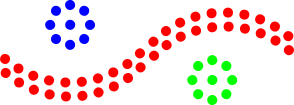
\includegraphics[scale=0.5]{images/dbscan.pdf}
  \caption[Clustering using the DBSCAN algorithm]{Clustering using the DBSCAN algorithm.}
  \label{images:dbscan}
\end{figure}


\section{Document Summarisation}
\label{sec:document-summarisation}

The problem of API summarisation could be linked to the document summarisation one. In fact, it could be viewed as a multi-document summarisation task where, according to \nolink{\citeauthor{Aliguliyev:2010}} \cite{Aliguliyev:2010}, the intention is to create a compressed version of a given collection of documents, that provides useful information to the users. Multi-document text summarisation has been an emerging field throughout the last 15 years. The \textit{Document Understanding Conference}\footnote{\url{http://www-nlpir.nist.gov/projects/duc/index.html}} (DUC), organised since 2001\footnote{DUC is now part of the \textit{Text Analysis Conference} (TAC).}, has been the major forum for comparing summarization systems, while it also included the \textit{multi-document summarization task}, with the purpose of creating fixed-length summaries, for a set of given documents.

When summarising an API, the collection of documents refers to the source code repository that is going to be mined, while the compressed version is in the form of API call sequences, or even better of snippets. A common approach in multi-document summarisation, is to leverage unsupervised techniques, in order to cluster similar sentences. 

For instance, \nolink{\citeauthor{Wang:2008}} make use of semantic analysis, with the purpose of computing similarities between sentences, which they then cluster. This is followed by the retrieval of the most informative sentences from each cluster, which are going to form the summary. Similarly, \nolink{\citeauthor{Boros:2001}} \cite{Boros:2001} use a combination of hierarchical and non-hierarchical clustering techniques, with the aim of partitioning a set of sentences into clusters, with each of them containing sentences covering only a single topic. A more recent approach is the one presented in \cite{Liu:2012}, where \nolink{\citeauthor{Liu:2012}} build a deep learning model, in an attempt to efficiently solve the multi-document summarisation problem.

In addition to the multi-document summarisation problem, we are also going to consider the single-document summarisation task in this dissertation. This task aims to produce a summary of a single document. According to \nolink{\citeauthor{Aliguliyev:2010}} \cite{Aliguliyev:2010}, such a summary could be either \textit{extractive} or \textit{abstractive}. The first one includes these sentences that are considered important, in order for someone to understand the given document, while, according to \nolink{\citeauthor{Aliguliyev:2010}}, the generation of the second one ``usually needs information fusion, sentence compression and reformulation''.


\section{Source Code Summarisation}
\label{sec:source-code-summarisation}

Most of the systems that perform API mining so far present sequences of API method calls, rather than snippets, to the users. Although such sequences may seem interesting, they cannot adequately describe a source code example efficiently. On the other hand, presenting long snippets, such as the entire source code of the client methods that contain the mined sequences, may hinder the understanding of the target API, as these snippets usually contain several non-API relevant statements. This has prompted the authors of most recent publications in API usage mining to try to summarise usage examples \cite{Montandon:2013, Kim:2013}, or even to synthesise them, by combining information of similar snippets \cite{Buse:2012}.

In contrast to text summarisation which is a well-studied field, source code summarisation techniques have only emerged during the last years. These two fields have many similarities, though. \nolink{\citeauthor{Ramanujam:2016}} \cite{Ramanujam:2016} identify three characteristics of a good text summary; \textit{coverage}, \textit{coherence} and \textit{redundancy}. We could claim that both characteristics apply to source code, too. What differentiates, however, the process of text summarisation from that of source code summarisation is that a source code, in contrast to free text, contains semantic as well as structural information. Hence, simple approaches that leverage text summarisation techniques (e.g. $tf/idf$), and that are based on keywords, cannot be efficiently applied to source code as they neglect the semantic context.

Similarly to a single text document summary, the major goal of a code fragment summary is to present the main ideas in the original fragment in less space. There have been interesting studies that try to define what a good source code example, and by extension summary, is. For instance, \nolink{\citeauthor{Nasehi:2012}} \cite{Nasehi:2012} introduce the notion of the \textit{concise code}, which usually contains less than four lines of code, while replacing unnecessary details with placeholders (comments or ellipses). Moreover, \nolink{\citeauthor{Ying:2014}} \cite{Ying:2014} identify common summarisation practices (e.g. shortening identifiers or formatting code for readability) by  conducting user studies.

\nolink{\citeauthor{Ying:2013}} \cite{Ying:2013} introduce a novel way to summarise code fragments, by exploiting ML techniques. Their system trains a classifier, using feature vectors, that contain features which are either syntactic or even related to the query, in order to decide on whether a line of the given source code should be in the summary or not. This is an interesting approach, but a general-purpose one.

Instead, taking into consideration that, in the case of API usage mining, we are mainly interested in statements that contain API-relevant information, \nolink{\citeauthor{Kim:2013}} \cite{Kim:2013} exploit \textit{slicing}\footnote{There have been almost 35 years since \nolink{\citeauthor{Weiser:1981}} \cite{Weiser:1981} defined \textit{program slicing} as a method for isolating only the part of a program that is of interest to the user, based on a slicing criterion. Here, we are primarily interested in \textit{static slicing}, which does not take into consideration the execution of the program.} techniques, to extract only the semantically relevant -to the given API method- lines. In the same direction, \nolink{\citeauthor{Montandon:2013}} \cite{Montandon:2013} devise a summarisation algorithm, which uses \textit{forward} and \textit{backward slicing}\footnote{The purpose of \textit{backward slicing}, is to find these statements that contribute to the -information used in the- defined  criterion, while \textit{forward slicing} identifies the statements that are affected by that.} techniques, with the purpose of excluding the non-API statements. This seems a promising task-specific approach but, as we are going to explain during the analysis of our implementation, this could still result in undesirable redundancy.
\chapter{Existing Work on API Summarisation}
\label{chap:existing-work}

\section{Defining the Problem}
\label{sec:problem-definition}

As mentioned in \Cref{sec:hypothesis}, the problem we are facing in general is that of mining API usage patterns, which has been clearly described by \nolink{\citeauthor{Ishag:2016}} in \cite{Ishag:2016}. However, here we specifically define four main features that a system that performs API usage mining should exhibit. That is, given a -local- repository of Java source code files that are relevant to the target API, the system to be developed should be able to:

\begin{itemize}
\setlength\itemsep{0.1em}
\item[\featureyes] Consider the structure of the source code files
\item[\featureyes] Cluster similar usage examples
\item[\featureyes] Summarise the examples into concise and readable snippets
\item[\featureyes] Present a ranked list of snippets to the users
\end{itemize}

As revealed from the above features, our primary goal is to mine common usage snippets that are concise and readable, instead of mining and presenting frequent sequences of API method calls. In addition to that, we are going to explore ML and NLP techniques in order to approach the problem efficiently, many of which have not been applied to any systems before.

The most striking examples of similar systems that conduct API usage mining are analysed in the next two sections. We divide them into two categories; the first one consists of systems that present sequences, and the second one of these that present snippets to the users.


\section{Systems that Output Sequences}
\label{sec:sequence-systems}

One of the very first systems to mine API usage patterns has been the \textit{MAPO} system \citep{Xie:2006}. Its objective has been to generate usage patterns, that could then act as an index for the recommendation of code snippets. MAPO is an ordinary example of a system that performs frequent sequence mining. As regards the representation of the source code, the system firstly extracts API method call sequences from the given source code files. After that, MAPO clusters these sequences, on its most recent version \citep{Zhong:2009}, with the aim of improving the quality of the mined patterns. On its next step, the system combines the mined frequent call sequences -extracted using the \textit{SPAM} sequence miner \citep{Ayres:2002}- from each cluster, to produce patterns that are eventually presented to the users. The latest version of the MAPO system, accompanies the API sequences with their associated snippets. However, it is still more of a sequence-based approach, as it shows the source code of the client method without proceeding to any summarisation, while it also avoids to consider the structure of the snippets.

In \citep{Wang:2013} the authors argue that MAPO outputs a large number of usage patterns, many of which are moreover redundant. To overcome these issues, \nolink{\citeauthor{Wang:2013}} define \textit{scalability}, \textit{succinctness} and \textit{high-coverage} as the main characteristics by which an API miner should abide. Based on these characteristics, their \textit{UP-Miner} system focuses on qualitative usage patterns. Their approach includes a two-step clustering, as well as mining of frequent closed sequences -using the \textit{BIDE} algorithm \citep{Wang:2004}- in order to mine usage patterns of single API methods. Although the UP-Miner tool is able to extract even more rear patterns, which cannot be extracted by the MAPO system, we believe that the use of probabilistic graphs of API method calls, in order for the first system to present the results may confuse the users, who definitely prefer simpler ways for the presentation of such results (e.g. ranked lists).

A brand new system that introduces several novelties with the purpose of presenting API usage patterns, in the form of sequences, is presented in \citep{Fowkes2:2015}. \nolink{\citeauthor{Fowkes2:2015}} point out that most of the heavily used frequent sequence mining methods require multiple user-defined parameters, that need to be hard-coded, and which are additionally hard to tune. With the aim of avoiding manually given parameters, they present a near parameter-free probabilistic algorithm (\textit{PAM}), which is able to cluster method sequences, and to extract ``the most informative API call patterns''. In this way, \nolink{\citeauthor{Fowkes2:2015}} apply techniques used in statistics and in the ML field to source code. This is the first system to mine API calls at GitHub scale, and to evaluate using handwritten examples that exist in libraries' \texttt{examples} directory, as \textit{gold standards}\footnote{A \textit{gold standard} (also known as ``oracle example'') is supposed to be an ideal example, based on which the quality of other examples can be evaluated.}. Using examples written by the developers of a library to evaluate API miners seems a promising concept, that would enable the drawing of more objective conclusions, compared to the ones drawn from user studies. Additionally, using the libraries' \texttt{examples} directory allows the use of automatic evaluation methods, which would not usually be possible. We will dive more into this concept in \Cref{chap:evaluation}. Although the outcome of this system is a list of method sequences rather than of usage snippets, we are going to leverage techniques used in this paper.


\section{Systems that Output Snippets}
\label{sec:snippet-systems}

Instead of presenting API-relevant sequences to the users, many systems during the last years output snippets. A possible usage scenario of such systems includes the enrichment of the APIs' documentation.

Upon improving the documentation of a target API, \nolink{\citeauthor{Kim:2009}} \cite{Kim:2009, Κim:2010, Kim:2013} firstly exploit slicing techniques, in order to summarise snippets retrieved by the \textit{Koders}\footnote{Renamed to \textit{Black Duck Open Hub Code Search}, before being discontinued in June 2016.} CSE. Their summarisation algorithm preserves the lines of the source code that are relevant to the target API, using common backward and forward slicing. The next step is to represent the summarised snippets using feature vectors. For this task the system makes use of the \textit{DECKARD} clone detection algorithm \cite{Jiang:2007}, which is a tree-based similarity detection algorithm, that proposes vectors for approximating the semantic context of ASTs. \nolink{\citeauthor{Kim:2009}} feed this algorithm with Java source code elements, while they also include additional features, such as the frequency of the query API method, and the lines of code in the snippets. Having extracted the feature vectors, they then experiment with three different approaches, in order to organise the generated examples; the \textit{eXoaCluster} algorithm, that uses the $k$-means clustering technique to cluster similar usage examples, the \textit{eXoaRank} algorithm, which ranks the examples based on their probability/frequency, and the \textit{eXoaHybrid} algorithm, that combines both of the aforementioned approaches. A disadvantage of the \textit{eXoaDocs} system we identify is that the system is not really capable of mining frequent patterns that include multiple API method calls. This is based on the fact that their feature vectors do not include any such information. Thus, the system mainly targets usage examples of single API methods.

Another approach that is not quite common is that followed in \cite{Wang:2011}, where \nolink{\citeauthor{Wang:2011}} make use of the \textit{Google Search} web search engine, in order to find useful examples. The \textit{APIExample} tool extracts code snippets, as well as their surrounding text from webpages, with the purpose of forming usage examples. It then clusters\footnote{Here, only client methods that contain the same API calls are clustered together.} these examples, and ranks them using intra-cluster and inter-cluster ranking heuristics. However, this tool does not summarise the usage examples, while we could argue that the clustering technique used does not lead to significant reduction in the number of the collected examples.

A more recent system that is presented in \cite{Montandon:2013} is the \textit{APIMiner}\footnote{\url{http://apiminer.org/}}. One of the highlights of the first version of this system is the summarisation algorithm that has been implemented by the authors, which uses backward and forward slicing, in order to preserve only the API-relevant statements of a source code file. In its most recent version, which is based on the work presented in \cite{Borges:2014}, the APIMiner leverages association rule techniques, and uses an improved version of the summarisation algorithm, with the aim of resolving variable types, or adding abstractive comments. However, it does not cluster similar usage examples, and additionally, our investigation of the system, revealed that most of the examples show the usage of a single API method.

Even when slicing is employed in the aforementioned systems, mined examples often contain extraneous statements, as pointed out by \nolink{\citeauthor{Buse:2012}} \cite{Buse:2012}. Therefore, the authors introduce a novel system that synthesises representative and well-typed usage examples. To the best of our knowledge, this in the first system to synthesise abstract examples, which it then presents to the users. This system combines \textit{path sensitive data flow analysis}\footnote{According to \nolink{\citeauthor{Winter:2013}} \cite{Winter:2013}, in path sensitive data-flow analysis (or path-sensitive DFA), path information that reveals whether a path is feasible or not is collected, with the aim to report bugs from feasible paths only.}, clustering, and pattern abstraction, in order to present usage examples that are quite complete and abstract. The mined snippets include abstract naming, as well as helpful code, such as \texttt{try} and \texttt{catch} statements. However, the fact that the source code is represented using graphs makes the system really complex, and probably inefficient as pointed out in \citep{Wang:2013}.
\chapter{Conceptual Design Work}
\label{chap:conceptual-design-work}

\section{Overview}
\label{sec:conceptual-overview}

In this chapter we present our approach to the problem defined in \Cref{sec:problem-definition}, while justifying any design decisions made at any particular stage. At first, we clearly describe the input and output of the system. Then, we provide an overview of our approach, before explaining each step and decision separately.


\section{Input and Output of the System}
\label{sec:input-output}

In contrast to the majority of the systems that perform API usage mining, where the input of the system is usually a repository of source code files, as well as a class or a method of the target API, our system needs a slightly different input as this is described below:

\begin{description}
\item[Input] A repository of Java source code files (client code), as well as a \texttt{.arff} file, consisting of client methods, and of their associated API call sequences. Each row in the \texttt{.arff} file is in the form presented in \Cref{listings:arff-transaction}, where the \texttt{client\_method} (also called ``caller'') and any \texttt{API\_call\textsubscript{i}} (also called ``call'') are fully qualified names. A sample row in the \texttt{.arff} file for the \texttt{Twitter4J} API is shown in \Cref{listings:twitter4j-arff-transaction}.
\item[Output] A ranked list of Java snippets. An example is shown in \Cref{listings:exp3-hdbscan-top-snippets}.
\end{description}

\begin{figure}[h]
  \lstinputlisting[language=arff]{listings/ArffTransaction.arff}
  \vspace{-10pt}
  \caption[Transaction in the \texttt{.arff} file]{General form of a transaction in a \texttt{.arff} file.}
\label{listings:arff-transaction}
\end{figure}

\begin{figure}[h]
  \lstinputlisting[language=arff]{listings/Twitter4jArffTransaction.arff}
  \vspace{-10pt}
  \caption[Transaction in the \texttt{twitter4j.arff} file]{Transaction in the \texttt{twitter4j.arff} file.}
\label{listings:twitter4j-arff-transaction}
\end{figure}

As revealed by the input of our system, we aim to mine usage example for the entire target API, rather than for a single method or a class of it. However, an input in the latter forms would only involve filtering of the mined snippets.


\subsection{Justifying the Form of the Input}
\label{subsec:input-form}

Our decision to use a different input from that used in the literature, stems from the fact that our team has already created a well-formed local corpus of the top Java projects in GitHub\footnote{\url{http://groups.inf.ed.ac.uk/cup/javaGithub/}} \cite{Allamanis:2013}. This, at first, prompted us to use this corpus as the source of our system. 

Furthermore, taking into account the limited time for the elaboration of this dissertation, and the fact that there has already been some previous work on API usage mining from our team in \cite{Fowkes2:2015}, we decided to use the \textsc{Example} dataset presented in that work. This would allow us to spent more valuable time on the main task of mining patterns, rather than on that of finding relevant files in the GitHub Java corpus. This dataset includes popular libraries and frameworks that also contain an \texttt{examples} directory, which is moreover going to enable the comparison of our system's mined snippets with these handwritten examples. For each library, \nolink{\citeauthor{Fowkes2:2015}} have created a directory of source code files that import a class belonging a (sub)package of the library (client code), while they have also generated the aforementioned \texttt{.arff} files\footnote{The best-effort approach used to extract the API call sequences, and to generate the \texttt{.arff} file subsequently, is described extensively in \cite{Fowkes2:2015}, and is out of the scope of this dissertation.}.

We point out that, ideally, there would exist a mapping between the \texttt{.arff} transactions and their associated source code files. However, as this information was not available for the \textsc{Example} dataset, we created a script that uses a best-effort approach, in order to do this. Our approach uses the fully qualified name of each client method, with the aim of finding its source code file. When there are duplicate class files, (these are labelled: \texttt{Class.java}, \texttt{Class\_2.java}, \texttt{Class\_3.java}, etc), we parse the package declaration of each class file, and match it to that of the client method's one.


\section{Overview of the Proposed Methodology}
\label{sec:methodology-overview}

Our methodology may be summarised in the following points:

\newcommand\litem[1]{\item{\bfseries #1\\}}
\begin{enumerate}
\litem{Clean the \texttt{.arff} file} This step filters the \texttt{.arff} file, by removing any sequences that are not of interest, as we are going to explain in \Cref{sec:data-preprocessing}.
\litem{Cluster the sequences in the cleaned \texttt{.arff} file} In this step, we leverage clustering techniques, in order to cluster the API call sequences in the \texttt{.arff} file. We analyse the process in \Cref{sec:clustering-step}.
\litem{Select a fixed number of sequences from each cluster} This is a clustering postprocessing step, that selects the top sequences from each cluster, as briefly explained in \Cref{sec:sequence-selection}.
\litem{Generate a summarised snippet for the source code associated with each selected sequence} In this step we retrieve the source code files that are associated with the sequences that have been selected in the previous step, and generate a summarised snippet for each of them, by leveraging a summarisation algorithm we implemented. We explain the process followed, as well as the decision to implement our own summarisation algorithm, in \Cref{sec:snippet-generation}. 
\litem{Select a single summarised snippet from each cluster} In this step we use a tree edit distance metric, in order to select a single snippet from each cluster, as explained in \Cref{sec:select-snippet}.
\litem{Rank the selected snippets, based on their support} This is the final step, where we rank the snippets in order of decreasing support. This is described in \Cref{sec:results-presentation}.
\end{enumerate}


\section{Cleaning the \texttt{.arff} File}
\label{sec:data-preprocessing}

A crucial step that precedes the application of clustering techniques to the data is the preprocessing step, which basically refers to the appropriate cleaning, that aims to remove the data that could break down even a powerful clustering algorithm. However, data cleaning has not only to do with the clustering quality; it also refers to the removal of any data that is not of interest. In our case, we proceed to the following removals:

\begin{itemize}
\litem{Remove callers that refer to different versions of the same source code file} An identical caller name indicates a different version of the same file. We remove multiple versions of the same source code file, as we noticed that most of them are identical in terms of API call sequences, and that they would affect the clustering process. An example is shown in \Cref{listings:versions}.
\litem{Remove singleton sequences} These are the sequences that contain only a single API call. We claim that singletons do not contain any useful information, as they do not show any interaction between different API methods. An example is shown in \Cref{listings:singleton}.
\litem{Remove pseudo-singleton sequences} These are the sequences that contain only a single API method, which is invoked multiple times. An example is shown in \Cref{listings:identical}.
\litem{Removes unique\footnote{We define a \textit{unique sequence} as this sequence for which there is no other sequence that contains the same API calls, invoked in the same order. That is, there is no other identical sequence.} sequences, if specified so} An interesting decision here is that of whether to remove the sequences that are unique. Although the removal of the unique sequences would result to more tight clusters, we would probably miss rare patterns, while the fact that they are unique does not mean that they do not share API calls with other sequences. Based on this, we decided to have this feature as a parameter of the preprocessing step, and consider this on the evaluation of the system.
\end{itemize}

\begin{figure}[ht]
\lstinputlisting[language=arff]{listings/Versions.arff}
\vspace{-10pt}
\caption[Example indicating multiple versions of the same source code file]{Example indicating multiple versions of the same source code file.}
\label{listings:versions}
\vspace{-5pt}
\end{figure}

\begin{figure}[ht]
\vspace{-10pt}
\lstinputlisting[language=arff]{listings/Singleton.arff}
\vspace{-10pt}
\caption[Example indicating a singleton sequence]{Example indicating a singleton sequence.}
\label{listings:singleton}
\vspace{-5pt}
\end{figure}

\begin{figure}[ht]
\vspace{-10pt}
\lstinputlisting[language=arff]{listings/Identical.arff}
\vspace{-10pt}
\caption[Example indicating a pseudo-singleton sequence]{Example indicating a pseudo-singleton sequence.}
\label{listings:identical}
\vspace{-5pt}
\end{figure}


\section{Clustering the Sequences}
\label{sec:clustering-step}

In this section we analyse any design decisions that are related to the clustering process. For instance, we justify our decision to apply clustering techniques at this stage, as well as our decision to cluster the sequences using a distance matrix instead of a feature vector. In addition to that, we visualise the \texttt{Twitter4J} dataset, in order to investigate whether there is a clear notion of clusters. Finally, we provide a brief overview of the clustering techniques we implemented, which are going to be analysed extensively in the next chapter.


\subsection{Why Clustering at This Stage?}
\label{subsec:clustering-decision}

Our decision to use clustering techniques, and more specifically at this stage, is quite simple. At first, looking at the client code in \Cref{listings:cluster-snippet1,listings:cluster-snippet2}, we see that these two snippets are quite similar, while they contain the same API calls (these are highlighted appropriately). A clustering technique that is based on the API call sequences of the client code would cluster these two snippets together. Taking into account the large number of files in the repository, this seems a more efficient approach than a clustering technique that would consider the structure of the client code, too. After all, we take into consideration the structure of the clustered snippets at a next stage, as described in \Cref{sec:select-snippet}. Hence, this approach is a balance between time overhead and quality improvement.

\begin{figure}[h]
\lstinputlisting[language=Java,style=Java]{listings/ClusterSnippet1.java}
\vspace{-10pt}
\caption[Sample client code 1]{Sample client code where the API calls are highlighted.}
\label{listings:cluster-snippet1}
\end{figure}

\vspace{-10pt}

\begin{figure}[H]
\lstinputlisting[language=Java,style=Java]{listings/ClusterSnippet2.java}
\vspace{-10pt}
\caption[Sample client code 2]{Sample client code that contains the same API calls with the client code presented in \Cref{listings:cluster-snippet1}.}
\label{listings:cluster-snippet2}
\end{figure}

\vspace{-20pt}

\subsection{Feature Vector vs Distance Matrix}
\label{subsec:feature-extraction}

The common input of a clustering algorithm is a feature vector that is generated from the data. While clustering using a feature vector has the advantage that one can apply almost every clustering technique on the vector, we identify a few problems here; one of them is that the designer should decide on the features to be used. In our case, a feature vector could be a boolean vector, where each future would represent a unique API method\footnote{Notice that we are talking about API methods and not about API calls; an API method may be called multiple times.}. As we understand, in this way we would represent the data as itemsets, rather than as sequences. The latter could be achieved by defining additional features that reveal the order in which the API methods are invoked.

Instead of generating a feature vector, probably the most common way to cluster sequences is to compute a distance/similarity matrix, using a sequence distance/similarity metric, and then cluster the sequences using this matrix. This approach cannot leverage algorithms that are based on Euclidean distances (such as the $k$-means one), but the majority of clustering techniques can be modified in order to receive a distance matrix instead of a feature vector as an input\footnote{We point out here that, while pre-computing a distance matrix would result to higher memory usage, it would also lead to lower computational/time complexity, as any clustering algorithm would compute this information at some point.}. In order to compute the similarity between any two sequences we tried several metrics, and we are going to analyse the most consistent of them in the next chapter. Our conclusion is that there is no significant difference in the results when using the one or the other, and thus we decided not to consider this as a parameter during the evaluation of the system.


\subsection{Visualising the Data}
\label{subsec:data-visualisation}

Considering that we now have a representation of our data, it would be interesting to try to visualise this. Taking into account the high-dimensional nature of the data, this would be tricky enough, though. Dimensionality reduction methods like the popular \textit{PCA} or the \textit{Isomap} kernels would not work in our case, as the data seem quite sparse. A technique that is usually applied in high-dimensional sparse data is this of the \textit{t-SNE} method \cite{Maaten:2008}, which converts similarities between data points to joint probabilities. Trying to visualise the data\footnote{At this step, we do not remove unique sequences in order to have a comprehensive picture of our data.} using the implementation of the t-SNE algorithm, which is part of Python's \texttt{scikit-learn} library\footnote{\url{http://scikit-learn.org/stable/modules/generated/sklearn.manifold.TSNE.html}}, we noticed that, although there were a few dense areas, most of the sequences are unique and similar to multiple other sequences, a fact that may confuse the t-SNE algorithm. A possible visualisation of the data is shown in \Cref{images:tsne-plot}. We should point out here that the visualisation is highly affected by several factors, such as the sequence similarity metric, and the parameters used in the t-SNE algorithm. In any case, this plot indicates that it is difficult enough to predict the number of clusters -even with the use of popular metrics such as the \textit{silhouette coefficient} or the \textit{Elbow} method as we ascertained later- as there are no clear, with respect to cohesion and even more to separation, clusters in the data.

\begin{figure}[h]
  \centering
  \includegraphics[scale=0.4]{images/tsne-plot}
  \caption[Plotting the data using the \textit{t-SNE} technique]{Plotting the sequences of the \texttt{Twitter4J} API using the \textit{t-SNE} algorithm.}
  \label{images:tsne-plot}
\end{figure}


\subsection{Applying Clustering Techniques}
\label{subsec:clustering-techniques}

Regarding the clustering techniques that have been investigated in the current project, although we tried several algorithms, two of them have been proven promising, and thus we decided to evaluate two different versions of the system, with respect to the clustering algorithm used. The first one uses an implementation of the $k$-medoids algorithm, the basic version of which has been described in \Cref{subsec:k-medoids}, while the second one is a hierarchical version of the DBSCAN algorithm (named \textit{HDBSCAN}, and introduced in \cite{Campello:2013}). We also tried different approaches for the initialisation of the medoids for the $k$-medoids technique, and implemented the $k$\verb!++! technique which has been proven more efficient than a random initialisation for this task. Regarding the number of clusters, we tried to predict them using popular methods, including the Elbow or the silhouette coefficient ones, however, none of them showed any cut-off point, and thus we decided to hard-code this parameter, using our intuition.

In any case, the result of the clustering process will be a clustered version of the \texttt{.arff} file. An example is shown in \Cref{listings:arff-clustering}, where the callers whose sequences have been clustered together are highlighted using the same colour.

\begin{figure}[h]
  \lstinputlisting[language=arff,style=arff]{listings/SequenceClustering.arff}
  \vspace{-10pt}
  \caption[Clustered \texttt{.arff} file]{Clustered version of the \texttt{.arff} file.}
\label{listings:arff-clustering}
\end{figure}


\section{Selecting the Most Representative Sequences}
\label{sec:sequence-selection}

The next step after clustering the sequences, is to retrieve the source code of the most representative sequences of the clustering. A simple solution would be to select the most representative sequence of each cluster (the ``medoid'' sequence in the case of the $k$-medoids algorithm, or probably the sequence with the highest intra-cluster support for the HDBSCAN algorithm), and then retrieve and present its associated source code to the user. However, we decided to consider more than one sequences from each cluster; this includes any sequence that is identical to the most representative one. This would allow us to take into account the structure of the source code files that contain the same API calls, in order to select the one with the most common structure, as we are going to explain in \Cref{sec:select-snippet}, and mainly in \Cref{sec:snippet-selector}. We decided to use a fixed number for the maximum number of sequences to be retrieved from each cluster, which is a balance between time overhead and quality improvement.


\section{Generating Summarised Snippets}
\label{sec:snippet-generation}

For each of the selected sequences, we retrieve its associated source code, and generate a summarised version of it. The main steps of this process are shown below:

\begin{enumerate}
\item Extract the body of the client method associated with the mined sequence.
\item Summarise the source code of the previous step, using the summarisation algorithm that has been implemented as part of the current dissertation.
\end{enumerate} 

Regarding the first step, our initial approach has been to get the subtree of the \textit{Longest Common Ancestor} (LCA) of the statements where the API methods are invoked, and present this to the user. However, we decided to go even further and implement a summarisation algorithm, which is analysed extensively in the next chapter. Our decision on proceeding to such an implementation is explained in 
\Cref{subsec:summarisation-algorithm-decision}.


\subsection{Implementing a Novel Summarisation Algorithm}
\label{subsec:summarisation-algorithm-decision}

After investigating summarisation algorithms that have been implemented as part of systems that perform API usage mining, we realised that the majority of them fails either in terms of quality, or in terms of time complexity.

More specifically, general-purpose algorithms, like the one presented in \cite{Ying:2013} cannot efficiently produce a summarised version of a client code. The primary reason is that they mainly include syntactic features, without giving the appropriate weight to the statements that are relevant to the API. Additionally, most of them summarise a code fragment based on lines rather than on statements, a fact that could lead to incomplete snippets.

Even the algorithms that are claimed to be specialised in the task of API usage mining, could result to high computational complexity, while the summarised code may still contain numerous statements, most of which can be considered redundant. For instance, the algorithm presented in \cite{Montandon:2013} makes use of backward and forward slicing techniques, which inevitably lead to a high time overhead, taking into account that the backward and forward slicing is executed multiple times. Additionally, a client code in which the variables used in statements that are relevant to the API, are also used in several statements that are not relevant to the API, could not be efficiently summarised by this algorithm. As an example, the algorithm would not remove -almost- any of the statements in the client code presented in \Cref{listings:without-summariser}.

Based on the above, we proceeded to the implementation of a novel summarisation algorithm, which is going to be analysed in the next chapter. Our algorithm produces the summarised snippet presented in \Cref{listings:with-summariser}, when it is applied to the client code in \Cref{listings:without-summariser}. As we can see, it successfully produces a summarised version of the original client code, which is both readable and concise.


\section{Selecting the Most Representative Snippets}
\label{sec:select-snippet}

Until this stage we have generated summarised snippets for the top files of each cluster. However, we have not yet taken into account the structure of the snippets. In an attempt to do so, we decided to leverage a tree edit distance metric\footnote{\nolink{\citeauthor{Pawlik:2016}} \cite{Pawlik:2016} define the \textit{tree edit distance} between two trees as the minimum-cost sequence of node edit operations that transform one tree into another.} on this step. Using such a metric, we are then able to select the most representative snippet among the summarised snippets associated with the top files of each cluster. This can be achieved by creating, for each cluster, a distance matrix that stores the tree edit distance between any two top snippets of the cluster, and then selecting the snippet with the minimum sum of distances in its cluster's matrix.

Analysing the concept above, assuming $N$ top snippets from each cluster, an $N\times N$ distance matrix is created, as shown in \Cref{tables:apted-distance-matrix}. The tree edit distance between the $i_{th}$ and $j_{th}$ snippet is stored in position $ij$ of the matrix. Then, the sum of distances associated with the most representative snippet of this cluster is highlighted.

\begin{table}[ht]
\centering
\small
\caption[Distance matrix computed using a tree edit distance metric]{Distance matrix that stores the tree edit distance between any two top snippets of a cluster. The index associated with the most representative snippet is coloured blue.}
\label{tables:apted-distance-matrix}
\input{tables/apted-distance-matrix.tex}
\end{table}

The computation of the tree edit distance between any two Java snippets is analysed in the next chapter.


\section{Ranking the Selected Snippets}
\label{sec:results-presentation}

The order in which the results are shown to the users plays a crucial role for systems that perform API usage mining. Presenting a bag of snippets would lead to users dissatisfaction, as the number of these snippets may be quite large. This would require the users to spend enough time, in order to find for instance the most popular snippets. Considering that most of the systems use the support of the sequences/snippets in order to rank them accordingly, we worked in the same way.

Taking into account that there is no trivial way to compute the support for a source code file, we consider the API call sequence of each mined snippet. More specifically, if the API call sequence of a mined snippet is a subsequence of the API call sequence of a file in the repository, then we claim that the latter file supports the mined snippet. An example that shows the API call sequence of a mined snippet, and that of a file in the mined repository that supports it, is shown in \Cref{fig:support}.

\begin{figure}[h]
\ffigbox
{%
  \begin{subfloatrow}[2]
  \ffigbox[\FBwidth]
    {\caption{}\label{listings:support1}}{\lstinputlisting[language=APTED,style=APTED]{listings/Support1.txt}}
  \hspace{1em}%
  \ffigbox[\FBwidth]
    {\caption{}\label{listings:support2}}{\lstinputlisting[language=APTED,style=APTED]{listings/Support2.txt}}
  \end{subfloatrow}}
  {\caption[Support of the mined snippets]{API call sequence (\subref{listings:support1}) of a mined snippet, (\subref{listings:support2}) of a file in the repository that supports the mined snippet. The API call sequence of the mined snippet is a subsequence (highlighted API calls) of the file in the repository.}
\label{fig:support}}
\end{figure}
\vspace{-15pt}

Having computed the support of each mined snippet, we then sort the snippets in descending order of support.

\chapter{Implementation}
\label{chap:implementation}

Having briefly analysed our approach to the problem, as well as the appropriate decisions we made, we can now proceed to the analysis of the actual implementation of our system.


\section{System Overview}
\label{sec:system-overview}

\begin{figure*}[ht]
\centering
\includegraphics[width=0.9\textwidth]{images/system}
\caption[The architecture of the system]{The architecture of the system.}
\label{images:API-summariser}
\vspace{-2pt}
\end{figure*} 

The architecture of the system is illustrated in \Cref{images:API-summariser}. As depicted, the system comprises the below mentioned components:

\begin{description}
\item[AST Extractor] Extracts the ASTs of the files in the repository.
\item[Data Cleaner] Cleans the \texttt{.arff} file and keeps only the API call sequences that are going to be clustered. 
\item[Clustering Preprocessor] Creates a distance matrix for the sequences, using a sequence distance metric.
\item[Clustering Engine] This is the primary component of the clustering process. It clusters the sequences using the distance matrix and a clustering technique, and stores the results in data structures and files.
\item[Clustering Postprocessor] This component receives the clustering results and identifies the most representative sequences of each cluster. It then retrieves their associated ASTs, which have been extracted by the \text{AST Extractor} component, and feeds them to the \textit{Snippet Generator} component.
\item[Snippet Generator] Generates summarised snippets for the files retrieved by the \textit{Clustering Postprocessor} component, by leveraging the summarisation algorithm.
\item[Snippet Selector] Selects the most representative snippet among the generated snippets of each cluster, based on a tree-edit distance.
\item[Ranker] Ranks the selected snippets based on their support.
\end{description}


\section{AST Extractor}
\label{sec:ast-extractor}

This component extracts the ASTs of the source code files in the repository, which are then used by the \textit{Snippet Generator} component, in order to generate summarised snippets. In order to extract the ASTs, we make use of the \texttt{srcml}\footnote{\url{http://www.srcml.org/about-srcml.html}} tool, which converts Java source code to the \textit{srcML} format. The srcML format is an XML representation for source code, where the mark-up tags identify elements of the abstract syntaxt for the language. An example of the AST extracted by the srcml tool, for a given Java source code, is presented in \Cref{sec:srcml-example}.


\section{Data Cleaner}
\label{sec:data-cleaner}

This component receives the content of the \texttt{.arff} file which, as described in \Cref{sec:input-output}, comprises of client methods and their associated API call sequences, and proceeds to the following modifications, as described in \Cref{sec:data-preprocessing}:

\begin{itemize}
\setlength\itemsep{1pt}
\item Removes callers that refer to different versions of the same source code file.
\item Removes singleton and pseudo-singleton sequences.
\item Removes unique sequences, if specified so by the appropriate parameter.
\end{itemize}

The result of this component is an updated version of the original dataset.

\vspace{-10pt}
\section{Clustering Preprocessor}
\label{sec:clustering-preprocessor}

This component creates a distance matrix, where the distance between any two sequences is stored. The distance metrics that have been implemented in order to compute the distance between any two sequences $S_1$ and $S_2$ are analysed below. Note that both distances are normalised in the range ${[}0.0$,$1.0{]}$.

\vspace{10pt}
\noindent
A. \textit{\underline{LCS distance}}
\vspace{5pt}

This metric makes use of the \textit{Longest Common Subsequence} (LCS) between two sequences, in order to compute their distance. The formula of the \textit{LCS distance} is shown in \Cref{eq:lcs-distance}.
%
\begin{align}
 \label{eq:lcs-distance}
 \centering
  LCS\_dist\left( S_1, S_2 \right) = 
  1 - 2\cdot\frac{ \left| LCS\left( S_1, S_2 \right) \right|}
       {\left| S_1 \right| + \left| S_2 \right|}
\end{align}
%
where $\left|LCS\left( S_1, S_2 \right) \right|$ is the length of the LCS between the two sequences.

As an example, given two sequences $S_1 = BAACD$ and $S_2 = AACBDE$, it holds that $LCS(S_1,S_2) = AACD$, and thus $\left|LCS\left( S_1, S_2 \right) \right| = 4$. Then, the LCS distance is:
%
\begin{align*}
 \centering
  LCS\_dist\left( S_1, S_2 \right) = 
  1 - 2\cdot\frac{ 4}
       {5 + 6} \simeq 0.27
\end{align*}
%
\vspace{10pt}
\noindent
B. \textit{\underline{SeqSim distance}}
\vspace{-2pt}

The \textit{SeqSim} metric is a sequence similarity metric that is based on \textit{n-grams}\footnote{Given a text sequence, an \textit{n-gram} is a contiguous sequence of $n$ items from the given sequence. According to the $n$ value, we may have \textit{unigrams} ($n=1$), \textit{bigrams} ($n=2$) and so on.}, which has been introduced in \cite{Wang:2013}. At first, the authors define the n-gram set $G(S)$, for a sequence $S(s_1s_2 ... s_n)$, as the collection of \textit{unigrams}, \textit{bi-grams}, ... , \textit{n-grams} of $S$, as shown in \Cref{eq:n-grams}:
%
\begin{align}
 \label{eq:n-grams}
  \begin{split}
    G(S) = 
    \lbrace s_1,s_2 ..., s_n,\;\; s_1s_2, s_2s_3 ..., s_{n-1}s_n,\;\; ...,\;\; s_1s_2...s_{n-1}, s_2s_3...s_{n-1}s_n, \\
    s_1s_2...s_{n-1}s_n\rbrace
  \end{split}
\end{align}
%
Then, the distance between $S_1$ and $S_2$ is computed using the formula in \Cref{eq:seqsim}.
%
\begin{equation}
 \label{eq:seqsim}
 \centering
  SeqSim\_dist\left( S_1, S_2 \right) = 
  1 - \frac{ \sum_{i} Weight(g_\cap^{i}) }
       { \sum_{i} Weight(g_\cup^{i}) }
\end{equation}
%
where $G_\cap = G(S_1)\cap G(S_2)$, $G_\cup = G(S_1)\cup G(S_2)$, $g_\cap^{i} \in G_\cap$, $g_\cup^{i} \in G_\cup$, and\\$Weight(g_\cap^{i})$, $Weight(g_\cup^{i})$ are equal to the length of $g_\cap^{i}$ and $g_\cup^{i}$, respectively.


As an example, given two sequences $S_1 = BAACD$ and $S_2 = AACBDE$:
%
\begin{align*}
  G(S_1) &= \lbrace B,A, ..., D,\;\; BA, AA ..., CD,\;\; ...,\;\; BAAC, AACD,\;\; BAACD\rbrace \\
  G(S_2) &= \lbrace A,A, ..., E,\;\; AA, AC ..., DE,\;\; ...,\;\; AACBD, ACBDE,\;\; AACBDE\rbrace \\
  G_\cap &= \lbrace A,B,C,D,\;\; AA,AC,\;\; AAC\rbrace \\
  G_\cup &= \lbrace A,B,...,E,\;\; BA,AA,...DE,\;\;...,BAACD,AACBD,ACBDE,\;\; AACBDE\rbrace
\end{align*}
%
which leads to:
%
\begin{align*}
  SeqSim\_dist\left( S_1, S_2 \right) &= 
  1 - \frac{ Weight(A) + Weight(B) +... + Weight(AAC)}
       { Weight(A) + Weight(B) +... + Weight(AACBDE) } \\
       &= 1 - \frac{ 1 + 1 +... + 3}
       { 1 + 1 +... + 6 } \simeq 0.86
\end{align*}
%
\vspace{15pt}
\noindent
C. \textit{\underline{Jaccard distance}}
\vspace{-10pt}

We have also implemented the \textit{Jaccard} distance. This is basically an itemset distance metric, a fact that makes it not so accurate as the two aforementioned metrics, but it is far more efficient, in terms of computational complexity, and thus it may be used for large datasets. Its formula is presented in \Cref{eq:jaccard}.
%
\vspace{1.5ex}
\begin{equation}
 \label{eq:jaccard}
 \centering
  Jaccard\_dist\left( S_1, S_2 \right) = 
  1 - \frac{ \left| S_1 \cap S_2 \right|}
       {\left| S_1 \cup S_2 \right|}
  \vspace{1.5ex}
\end{equation}
%
As an example, given two sequences $S_1 = BAACD$ and $S_2 = AACBDE$:
%
\vspace{4pt}
\begin{align*}
  Jaccard\_dist\left( S_1, S_2 \right) = 
  1 - \frac{ \left| \lbrace A, B, C, D\rbrace \right|}
       {\left| \lbrace A, B, C, D, E\rbrace \right|} = 1 - \frac{4}{5} = 0.2
  \vspace{15pt}
\end{align*}
%
\Cref{tables:sequence-similarity} shows a few indicative examples that point out the differences between the aforementioned metrics. As we can see, the \textit{Jaccard\_dist} metric may overestimate the similarity between the sequences, while the \textit{SeqSim\_dist} may underestimate it, a fact that could lead to a quite dense or sparse distance matrix respectively. It seems that the \textit{LCS\_metric} provides a balance between the other two metrics. For this reason, we decided to use this metric in the versions of the system that are going to be evaluated.

\begin{table}[ht]
\centering
\small
\caption[Sequence distance metrics examples]{Examples indicating the differences between the various sequence distance metrics that have been implemented.}
\label{tables:sequence-similarity}
\begin{tabular}{lllll}
\toprule
$S_1$ & $S_2$ & $LCS\_dist$ & $SeqSim\_dist$ & $Jaccard\_dist$\\
\midrule
ABC & ABC & 0.00 & 0.0 & 0.00 \\
AB & CDE & 1.00 & 1.00 & 1.00 \\
ACBD & ABDC & 0.25 & 0.82 & 0.00 \\
BAACD & AACBDE & 0.27 & 0.86 & 0.20 \\
AAAB & AAB & 0.14 & 0.44 & 0.00 \\
\bottomrule
\end{tabular}
\end{table}

The outcome of this component is an $N\times N$ table, where $N$ is the number of the sequences. Each sequence is assigned a unique id and, as a result, the value stored in the index $i,j$ of the table is the distance between the $i_{th}$ and the $j_{th}$ sequences\footnote{Although we use a \textit{redundant} (also called \textit{full} or \textit{complete}) distance matrix, we only need the upper triangular part -or even the lower one, as the first one is the transpose of the second one- of the distance matrix, taking into account that this is a symmetric matrix. A more efficient approach would use a \textit{condensed} distance matrix, which does not contain any redundancy.}.


\section{Clustering Engine}
\label{sec:clustering-engine}

The \textit{Clustering Engine} component implements the clustering techniques that could be used in order to cluster the sequences. Although we have integrated/implemented several clustering algorithms, we are going to analyse only the two that are used in the actual implementation. These include an implementation of the $k$-medoids algorithm, as well as the HDBSCAN\footnote{\url{https://github.com/lmcinnes/hdbscan}} algorithm \cite{Campello:2013}.

This component receives the distance matrix as input, and clusters the sequences using one of the implemented clustering techniques, which are analysed in this section.


\subsection{\texorpdfstring{$k$}{k}-medoids Implementation}
\label{subsec:k-medoids-implementation}

The implementation of the $k$-medoids algorithm is based on the one presented in \cite{Bauckhage:2015}. We have also implemented the concept behind the $k$\verb!++! initialisation, in order to predict the initial medoids more efficiently. A simplified pseudocode of the $k$-medoids algorithm that has been implemented is shown in \Cref{algorithms:k-medoids}, while the pseudocode of the $k$\verb!++! initialisation technique is presented in \Cref{algorithms:k++}.

\begin{algorithm}[h]
\small
\caption[$k$-medoids]{$k$-medoids}
\label{algorithms:k-medoids}
\begin{algorithmic}[1]
\Procedure{$k$-medoids}{$k$, $max\_iter$}
    \State Initialise $k$ medoids using the $k$\verb!++! initialisation technique
	\Repeat
		\State Assign each point to its closest medoid's cluster
		\State Update medoids by computing the mean of each cluster and getting the data point whose distance to the mean is the minimum one
	\Until{medoids do not change or $max\_iter$ reached}
\EndProcedure
\end{algorithmic}
\end{algorithm}

\begin{algorithm}[h]
\small
\caption[$k$\texttt{++}]{$k$\texttt{++}}
\label{algorithms:k++}
\begin{algorithmic}[1]
\Procedure{$k$\texttt{++}}{$k$}
    \State Initialise the first medoid randomly
	\Repeat
		\State Create a distance matrix $D$ which stores, for each data point, its distance from its closest medoid
		\State Choose the data point $i$ as the next medoid, uniformly, at random, with probability $\frac{D(i)}{\sum_{i \in data} D(i)}$
	\Until{$k$ medoids have been chosen}
\EndProcedure
\end{algorithmic}
\end{algorithm}


We have implemented the $k$-medoids algorithm in a similar way to that used in the \texttt{sklearn.cluster} class of the Python's \texttt{scikit-learn} library, which includes several implementations of clustering techniques. That is, we created a class named \texttt{KMedoids}, which includes a \texttt{fit} method, that receives the distance matrix as a parameter and calls the \texttt{static} \texttt{k\_medoids} function. The class can be instantiated and initialised using several parameters, including the number of clusters, the maximum number of iterations, and the initialisation technique to be used (either the $k$\verb!++! technique, or a random, or even a fixed initialisation that makes use of a given array). The algorithm returns the medoids and the labels that indicate the clusters to which the data points have been assigned.

The main differences between our implementation and the one presented in \cite{Bauckhage:2015} are summarised below:

\begin{itemize}
\item We have implemented the $k$\verb!++! initialisation in order to better predict the initial medoids, while we also provide the option of a predefined initialisation, given an array which comprises of the initial medoids.
\item Our algorithm avoids the creation of empty clusters. This is mainly a problem when the random initialisation is passed as an option, as the implementation in \cite{Bauckhage:2015} does not prevent from selecting identical data points as the initial medoids. Such a selection would lead to empty clusters and we avoid this by excluding identical data points from the random selection.  
\item We have implemented an additional criterion in order to decide on whether the algorithm has converged or not; this checks whether the members of the clusters have been assigned to a different cluster during the last iteration, rather than whether the medoids have been modified during that iteration. However, this option does not to show any real difference in the results for the datasets we use, and thus we decided to exclude it from the evaluation.
\end{itemize}


\subsection{HDBSCAN Implementation}
\label{subsec:hdbscan-implementation}

As regards the \textit{HDBSCAN} algorithm \cite{Campello:2013}, it is a hierarchical version of the DBSCAN algorithm, which has been described in \Cref{subsec:DBSCAN}, that varies the $Eps$ parameter, and integrates the result to find a clustering that gives the best stability over this parameter. This allows HDBSCAN to find clusters of varying densities (unlike the basic DBSCAN algorithm), and to be more robust to parameter selection.

There is already a high performance implementation of the HDBSCAN algorithm written in Python by Leland McInnes\footnote{\url{https://github.com/lmcinnes/hdbscan}}, and thus we decided to make use of this implementation.

\Cref{algorithms:hdbscan} summarises the basic steps of the algorithm, as these are described in the original paper, as well as in the documentation of the implementation we use\footnote{\url{http://nbviewer.jupyter.org/github/lmcinnes/hdbscan/blob/master/notebooks/How\%20HDBSCAN\%20Works.ipynb}}. For the definition of the terms used in \Cref{algorithms:hdbscan}, as well as for a deeper analysis of the algorithm, we encourage the reader to consider the original paper, as any further explanation is beyond the scope of this dissertation.

\begin{algorithm}
\small
\caption[HDBSCAN]{HDBSCAN}
\label{algorithms:hdbscan}
\begin{algorithmic}[1]
\State Compute the \textit{mutual reachability distance} between all data points
\State Create the \textit{Mutual Reachability Graph} (MRG), a weighted graph with the data points as vertices, and an edge between any two points with weight equal to the mutual reachability distance of those points
\State Compute the \textit{Minimum Spanning Tree} (MST) of the MRG via \textit{Prim}'s algorithm
\State Convert the MST into an hierarchy of connected components
\State Condense the MST using the $min\_cluster\_size$ parameter
\State Compute the \textit{stability} of each cluster and extract a flat, non-overlapping partition, that maximises the sum of these stabilities.
\end{algorithmic}
\end{algorithm}

Regarding the complexity of the algorithm, \nolink{\citeauthor{Campello:2013}} note that, in case a data matrix is provided as input (as in our case), both the time and the space complexity are reduced to $\mathcal{O}(n^2)$.

Although this implementation does not have any required parameters, we set the \texttt{min\_cluster\_size} parameters to two. This parameter indicates the minimum number of data points that could form a new cluster (namely, the minimum size of each cluster).


\section{Clustering Postprocessor}
\label{sec:clustering-postprocessor}

The next component receives the clustering results and retrieves a maximum number of files from each cluster, in order to generates snippets. In our actual implementation, we use a fixed number of maximum files to be retrieved, which has been set to $n=5$, while we only retrieve the medoid of each cluster, and at most $n-1$ sequences that are identical to it. This would allow us to have more precise patterns, as choosing sequences that are not identical could probably result to quite dissimilar sequences.

This component feeds the \textit{Snippet Generator} component with the top files to be used in order to generate snippets.


\section{Snippet Generator}
\label{sec:snippet-generator}

Having clustered the sequences and selected the top files of each cluster, the next step is to generate succinct snippets for these files. This component makes use of the ASTs extracted by the \textit{AST Extractor} component. The process followed is analysed below:

\begin{itemize}
\item For each of the top files of the clusters, received by the \textit{Clustering Postprocessor} component, we retrieve its associated \texttt{.xml} file, that contains its AST representation.
\item We extract the part of the \texttt{.xml} file that refers to the client method of the top file, and more specifically, we extract the body of the client method. However, we also store any class variables, as well as the method's parameters, in order to be able to resolve variable types at a later stage.
\item For each snippet of the previous step, we generate a summarised snippet, using the summarisation algorithm that has been implemented. Actually, for each \texttt{.xml} file of the previous step, which includes the body of the client methods, we generate a summarised \texttt{.xml} file, and convert it back to Java source code, using the srcml tool.
\end{itemize}

As an example, the \texttt{.xml} file associated with the caller \texttt{twickery.web.code.\protect\\UserCode.name} is the one presented in \Cref{listings:srcml-java}, with the body of the client method associated with the caller being highlighted. Regarding the generated summarised snippet, we are going to analyse this process in the next subsection, and thus it is better to avoid to present any examples here\footnote{After all, the presented example contains only a single statement and it does not make sense to present a summarised version of it.}.


\section{Summarisation Algorithm}
\label{subsec:summarisation-algorithm}

The summarisation algorithm receives as parameters the root of the \texttt{.xml} file, the API calls invoked in the snippet that is associated with the \texttt{.xml} file, and the variables that have been defined in a previous part of the source code (class variables and method's parameters). It then summarises the snippet, using the process presented in \Cref{algorithms:summarisation-algorithm}, which is further analysed in this section.

\begin{algorithm}
\small
\caption[Summariser]{Summariser}
\label{algorithms:summarisation-algorithm}
\begin{algorithmic}[1]
\Procedure{Summarise}{$tree$, $API\_calls$, $decl\_vars$}
    \State $tree \leftarrow$ Preprocess($tree$)
    \State $API\_stmts$, $non\_API\_stmts \leftarrow$ ClassifyStmts($tree$, $API\_calls$)
	\State $decl\_vars \leftarrow$ GetLocDeclVars($tree$, $decl\_vars$)
	\State $tree \leftarrow$ RemNonAPIStmts($tree$, $non\_API\_stmts$)
	\State $decl\_vars \leftarrow$ FilterDeclVars($tree$, $decl\_vars$)
	\State $API\_decl\_vars \leftarrow$ GetAPIDeclVars($API\_stmts$)
    \State $API\_vars\_not\_read \leftarrow$ CheckAPIDeclVarsRead($API\_decl\_vars$, $API\_stmts$)
	\State Add a declaration statement for each $var \in decl\_vars$ in $tree$
    \State Add a descriptive comment for each $var \in API\_vars\_not\_read$ in $tree$
    \State Add descriptive comments for empty blocks in $tree$
\EndProcedure
\end{algorithmic}
\end{algorithm}

\begin{itemize}
\item \textit{Line 2} firstly removes any comments. Moreover, it replaces any \texttt{literal} nodes in the srcML format with their srcML type. This includes nodes of srcML type \texttt{string}, \texttt{char}, \texttt{number}, \texttt{null}, and \texttt{boolean}. Such replacements lead to more abstractive snippets.
\item \textit{Line 3} distinguishes between API statements and non-API statements, based on whether an API method is invoked or not in these statements, and stores the corresponding nodes in appropriate lists. An extensive analysis, as well as the pseudocode of this function is presented in \Cref{sec:summarisation-pseudocodes} (\Cref{algorithms:statements-classifier}).
\item \textit{Line 4} retrieves all the variables that are declared locally.
\item \textit{Line 5} removes all non-API statements by iterating the tree in reverse order (reverse bottom-up pre-order traversal).
\item \textit{Line 6} filters the list of the variables that are declared either locally or as class variables, by checking whether these are used in the summarised tree, as well as if they have already been declared at a previous point. In the latter case, there is no need to re-declare them. Note that this function is called after removing the non-API statements, in order to iterate over the summarised tree, rather than on the original one.
\item \textit{Line 7} retrieves the variables that are declared in API statements.
\item \textit{Line 8} checks whether the variables retrieved in the previous line are used only in non-API statements after that point, and keeps only these for which this statement holds true.
\item \textit{Line 9} adds declarations statements for all the variables retrieved in Line 6.
\item \textit{Line 10} adds descriptive comments in the form ``\texttt{Do something with var}'', where \texttt{var} is one of the variables retrieved in Line 8.
\item \textit{Line 11} finds empty blocks (as a result of no existing API statements in their body), and adds descriptive comments in the form ``\texttt{Do something}'', to improve the readability of the source code.
\end{itemize}

\section{Snippet Selector}
\label{sec:snippet-selector}

The \textit{Snippet Selector} component receives the generated snippets of the clusters and selects one of them from each cluster, to be presented to the users. The process followed in order to select the most representative snippet of each cluster has been analysed in \Cref{sec:select-snippet}. However, there we intentionally did not explain the way the tree edit distance between two Java snippets is computed, as we use a tool for this purpose.

That is, in order to compute the tree edit distance between any two snippets, we leverage the APTED\footnote{\url{http://tree-edit-distance.dbresearch.uni-salzburg.at/}} tool, which implements the AP-TED algorithm, introduced in \cite{Pawlik:2016}. The AP-TED algorithm reduces the time complexity of the first-naive tree edit distance implementation, proposed in \cite{Tai:1979}, from $\mathcal{O}(n^6)$ to $\mathcal{O}(n^2)$, while also achieving an $\mathcal{O}(n^2)$ space complexity.

The APTED tool computes the tree edit distance between two trees, which are represented in a form similar to that presented in \Cref{subsec:graph-mining}. For instance, a tree with a root node A, that has two children B and C, where B has a child D, is represented by the transaction below:
%
\begin{align*}
\{A\{B\{D\}\}\{C\}\}
\end{align*}
%
In order to create such a transaction for an \texttt{.xml} file which is in the srcML format, we take into account the elements' tags in the \texttt{.xml} file. An indicative example that illustrates the whole process is presented in \Cref{sec:apted}.

As regards the parameters of the tool, one can set the cost for any insertion, deletion or renaming operation. However, we use the default values for these parameters, where the cost is $1$ for any of these operations.


\section{Ranker}
\label{sec:ranker}

The previous component selects a single snippet from each cluster. Then, we need to rank the mined snippets, in order to present them to the users in an order that reveals their importance. The \textit{Ranker} component sorts the snippets based on their support, with respect to the files in the mined repository, as described in \Cref{sec:results-presentation}.

Finally, we apply the \textit{Artistic Style}\footnote{\url{http://astyle.sourceforge.net/}} formatter to the ranked snippets, in order to improve their readability. This formatter mainly fixes any improper indents and spacings, while ensuring consistent spacing (e.g. before all brackets) in the snippets. An example of the application of this tool to Java source code is presented in \Cref{sec:artistic-style}.
\chapter{Evaluation}
\label{chap:evaluation}

\section{Overview}
\label{sec:evaluation-overview}

As we have seen so far, several parameters are used in our implementation. For instance, one can enable or disable the preprocessing step that removes the unique sequences, or do the same for the summariser. Moreover, we have implemented two different clustering algorithms that may lead to different results, in terms of the sequences that are clustered together. This prompts us to evaluate different versions of the system which, however, should vary as little as possible with respect to the different conditions. Ideally, when evaluating between different versions of a system, these versions may only differ by a single parameter, in order to draw appropriate conclusions.

In the next section we are going to explain our decision to evaluate the system's results using the examples written by the developers of the libraries, rather than writing our own gold standard examples.

After that, we present the different versions that aim to be used for the evaluation of the system, as well as the dataset used. Then, we divide the evaluation process into several experiments where, for each one, we clearly point out the hypothesis that is going to be tested. This step-by-step evaluation process will enable us to evaluate different aspects of the system and of the results. Additionally, the last experiment intends to evaluate the key hypothesis of the current dissertation.

We decided to use only the \texttt{Twitter4J} dataset in the conducted experiments, as we noted that, even when using this single dataset, we draw numerous interesting conclusions. Moreover, the hypotheses defined in the experiments may be well evaluated using this dataset.

To avoid any confusion, we firstly describe three main terms that are going to be used in the evaluation process.

\begin{description}
\item[Sequence] A sequence refers to an API call sequence. When this term is used in the evaluation metrics, this indicates the API call sequences of the snippets mined by our system.
\item[Snippet] A snippet refers to a Java code fragment mined by our system. The mined snippets are the results of our system.
\item[Example] An example refers to a handwritten Java code fragment, which is part of the \texttt{examples} directory of the target API. 
\end{description}


\section{Evaluating Using the \texttt{examples} Directory}
\label{sec:examples-evaluation}

In the majority of the publications in the field of API usage mining, the authors evaluate their systems with the aid of user studies. However, as we mentioned in \Cref{chap:introduction}, this inevitably leads to subjective results. Furthermore, \nolink{\citeauthor{Young:2005}} \cite{Young:2005} correctly point out that ``the human eye is a slow, expensive, and unreliable instrument for judging test outcomes''. This prompts us to use a more automatic way of evaluating our system. Taking into account that writing our own gold standard examples would also lead to subjective results, while it is moreover time consuming, a better approach would be to look for such gold standard examples in the internet. Fortunately, the developers of several APIs include such examples in their repositories. We believe that this is a really valuable information that could be usefully utilised for the evaluation of systems that perform API usage mining. In addition to that, the evaluation using handwritten examples that exist in the \texttt{examples} directory of the target libraries, has already been tested in \cite{Fowkes2:2015}, where the system under evaluation mines API call sequences. Therefore, we decided to use a similar methodology, with the intention of evaluating snippets rather than sequences. To the best of our knowledge, this is the first system to be evaluated using this methodology, and we hope that the outcome would be interesting enough, in the hope that this methodology will be used for the evaluation of similar systems in the future. After all, many popular authors in the field of IR insinuate that this field seems to lack of efficient and objective evaluation techniques \cite{Manning:2008}, and our approach may be helpful on that.


\section{Versions of the System Under Evaluation}
\label{sec:evaluation-versions}

\Cref{tables:evaluation-versions} illustrates the different versions of our system that are going to be considered during the evaluation process.

\begin{table}[ht]
\centering
\small
\caption[System versions]{Different versions of the system that are going to be considered under the evaluation process.}
\label{tables:evaluation-versions}
\begin{tabular}{lllll}
\toprule
\multirow{2}{*}[3pt]{Version} & Unique Sequences & Clustering & \multirow{2}{*}[3pt]{Summariser} \\[-5pt]
& Removal & Algorithm & \\
\midrule
$RemUniqNaivNoSum$ & ON & Naive & OFF \\
$RemUniqNaivSum$ & ON & Naive & ON \\
$KeepUniqNaivSum$ & OFF & Naive & ON \\
$KeepUniqKMedoidsSum$ & OFF & $k$-medoids & ON \\
$KeepUniqHDBSCANSum$ & OFF & HDBSCAN & ON \\
\bottomrule
\end{tabular}
\end{table}

As might be seen, the first parameter is related to the preprocessing step, and indicates whether the unique sequences are going to be removed or not. The second parameter is the clustering algorithm to be used, with the aim of clustering the API call sequences. The \textit{naive} algorithm has not been analysed in \Cref{chap:implementation}, as it purely clusters identical sequences together. In fact, there was no need to implement a different algorithm, as this could be seen as a $k$-medoids version, where the number of clusters equals the number of the non-identical sequences after the preprocessing step. The versions that use this algorithm are going to reveal whether a more powerful technique, that clusters similar rather than identical sequences, leads to better results. Finally, the summariser that leverages the implemented summarisation algorithm can be enabled or disabled in advance.

The values of the input parameters for the $k$-medoids and the HDBSCAN clustering algorithms are going to be presented in the experiments.


\section{Dataset}
\label{sec:evaluation-dataset}

As regards the dataset used, we make use of the \texttt{Twitter4J} dataset, which is part of the \textsc{Example} dataset, used in \cite{Fowkes2:2015}. This dataset targets the \texttt{Twitter4J} API, and summary statistics for the client code, as well as for the \texttt{examples} that are related to this dataset are presented in \Cref{tables:dataset-summary}. Taking into account that we are going to evaluate the results of the system using the handwritten examples in the \texttt{examples} directory as our gold standards, we decided not to split the dataset into a training and a test set. That is, the training set is the entire client code, while the test set includes the source code in the \texttt{examples} directory.

\begin{table}[ht]
\centering
\small
\caption[Dataset summary]{Summary of the \texttt{Twitter4J} dataset, which is part of the \textsc{Examples} dataset presented in \cite{Fowkes2:2015}.}
\label{tables:dataset-summary}
\begin{tabular}{lr}
\toprule
Attribute & Value \\
\midrule
No. client files & 549 \\
Client LOCs & 96,010 \\
No. API classes in client files & 81 \\
No. API methods in client files & 475 \\
No. transactions in the \texttt{.arff} file & 1,066 \\
No. singleton sequences in the \texttt{.arff} file & 367 \\
No. pseudo-singleton sequences in the \texttt{.arff} file & 39 \\
No. unique sequences in the \texttt{.arff} file & 585 \\
No. example files & 89 \\
Example LOCs & 5,458 \\
\bottomrule
\end{tabular}
\end{table}


\section{Evaluation Metrics}
\label{sec:evaluation-metrics}

In this section we present the metrics used in an attempt to evaluate the system. We make use of popular metrics related to the precision of the system, as well as to the coverage of the API methods in the dataset. Moreover, we define a metric that would enable us to evaluate whether presenting snippets rather than sequences is of more value to the developers. Furthermore, we make use of two quantitative metrics used in \cite{Buse:2012}, with the purpose of evaluating the summarisation algorithm. We point out that the expression $|x|$ is a shortcut for the expression ``number of $x$''.


\subsection{Precision Metrics}
\label{subsec:evaluation-precision}

Regarding the overall precision of the system, we define the $sequence\_precision$ and the $snippet\_precision$, in \Cref{eq:sequence-precision,eq:snippet-precision}, respectively.
%
\vspace{1ex}
\begin{equation}
 \label{eq:sequence-precision}
 \centering
  sequence\_precision = 
  \frac{ | \text{sequences contained in at least one example} | }
       { | \text{sequences} | }
\end{equation}
%
\begin{equation}
 \label{eq:snippet-precision}
 \centering
  snippet\_precision = 
  \frac{ \displaystyle\sum_{i=1}^{|snippets|}
   \frac{ | tokens\_snippet_i\, \cap \, tokens\_gold_{snippet_i} | }
  		{ | tokens\_snippet_i | } }
        { | \text{snippets} | }
 \vspace{2ex}
\end{equation}
%
where $tokens\_gold_{snippet_i}$ are the tokens in the example that best matches to $snippet_i$.

The $sequence\_precision$ metric is computed based on the API call sequences between a mined snippet and a handwritten example, while the $snippet\_precision$ takes into account the entire snippets. More specifically, the latter metric computes the overlap between a snippet and its most similar example, in terms of Java tokens. The process followed in order to extract the tokens and to compute the $snippet\_precision$ metric, is extensively analysed in \Cref{sec:snippet-based-metrics}.

We also define the $matched\_snippet\_precision$, in \Cref{eq:matched-snippet-precision}, with the intention of eliminating the effect of the snippets that have not been matched to any of the examples, to the value of the $snippet\_precision$ metric.
\vspace{1.5ex}
%
\begin{equation}
 \label{eq:matched-snippet-precision}
 \centering
  matched\_snippet\_precision = 
  \frac{ \displaystyle\sum_{i=1}^{m} 
  	\frac{ | tokens\_snippet_i \, \cap \, tokens\_gold_{snippet_i} | }
  		 { | tokens\_snippet_i | } }
       { m }
 \vspace{1.5ex}
\end{equation}
%
where $m$ is the number of snippets that match to at least one example.


\subsubsection{Evaluating the Precision of Ranked Results}
\label{subsubsec:evaluation-ranked}

Taking into account that our system returns a ranked list of snippets, we also make use of the \textit{precision at top $k$} ($precision@k$), which is also known as \textit{precision at cut-off $k$}. This metric indicates the precision calculated for the set of the top $k$ documents returned, and is heavily used for the evaluation of ranked documents\footnote{\url{http://nlp.stanford.edu/IR-book/html/htmledition/evaluation-of-ranked-retrieval-results-1.html}}. Such a metric would enable us to plot the precision for different values of $k$, while it would facilitate the comparison between versions of the system that return a different number of snippets. Based on this, and similarly to the precision metrics presented above, we firstly define the average sequence precision at top $k$ ($avg\_seq\_prec@k$), in \Cref{eq:avg-sequence-precision-atk}\footnote{Usually, there is a confusion on how the average at top $k$ is computed. In this evaluation, we use the formula in a similar way to that presented in \url{https://www.kaggle.com/c/avito-prohibited-content/forums/t/9584/average-precision-at-k-ap-k/50976\#post50976}}.
\vspace{1ex}
%
\begin{equation}
 \label{eq:avg-sequence-precision-atk}
 \centering
  avg\_seq\_prec@k = 
  \frac{ \displaystyle\sum_{i=1}^{k}
    seq\_prec@i }
       { k }
\end{equation}
%
where:
\vspace{1.5ex}
%
\begin{equation*}
 \label{eq:sequence-precision-ati}
 \centering
  seq\_prec@i = 
  \frac{ | \text{matched sequences at top $i$} | }
       { i }
 \vspace{1.5ex}
\end{equation*}
%
In a similar manner, the average snippet precision at top $k$ ($avg\_snip\_prec@k$) is defined in \Cref{eq:avg-snippet-precision-atk}.
\vspace{1.5ex}
%
\begin{equation}
 \label{eq:avg-snippet-precision-atk}
 \centering
  avg\_snip\_prec@k = 
  \frac{ \displaystyle\sum_{i=1}^{k}
    snip\_prec@i }
       { k }
 \vspace{1.5ex}
\end{equation}
%
where:
%
\vspace{1.5ex}
\begin{equation*}
 \label{eq:snippet-precision-ati}
 \centering
  snip\_prec@i = 
  \frac{ \displaystyle\sum_{j=1}^{i}
   \frac{ | tokens\_snippet_j\, \cap \, tokens\_gold_{snippet_j} | }
  		{ | tokens\_snippet_j | } }
        { i }
 \vspace{1.5ex}
\end{equation*}
%
Another metric used in order to evaluate the quality of the sequences, as well as of the snippets, is the \textit{Normalised Discounted Cumulative Gain\footnote{\url{https://www.kaggle.com/wiki/NormalizedDiscountedCumulativeGain}}}, which uses the graded relevance as a measure of usefulness. 

The formula of this metric is shown in \Cref{eq:ndcg}.
\vspace{1ex}
%
\begin{equation}
 \label{eq:ndcg}
 \centering
  nDCG_k = 
  \frac{ DCG_k } { IDCG_k }
\end{equation}
%
where:
\vspace{1ex}
%
\begin{equation*}
 \centering
  DCG_k = \displaystyle\sum_{i=1}^k
  \frac{  2^{rel_i}-1 } 
       { \log_2 (i+1) }
  \vspace{1.5ex}
\end{equation*}
%
\normalsize
and $IDCG_k$ is the maximum possible (ideal) $DCG$. Note that the value of $rel_i$ indicates the relevance of the $i_{th}$ recommended entity to the query.

Based on the above, we define the $sequence\_nDCG_k$ and the $snippet\_nDCG_k$. Regarding the value of $rel_i$, when computing the $sequence\_nDCG_k$, this is set to $1.0$ if the snippet's sequence is contained in at least one example, and to $0.0$ otherwise. This reveals that we consider it as a boolean variable. On the other hand, for the $snippet\_nDCG_k$, the value of $rel_i$ indicates the similarity of a snippet to the example it best matches to, and lies in the range [$0.0$,$1.0$]. The $IDCG_k$ is in both cases set to $1.0$.


\subsection{Metrics Used for the Evaluation of the Key Hypothesis}
\label{subsec:evaluation-key-hypothesis}

With the purpose of evaluating the key hypothesis of the current dissertation, which is that presenting snippets rather than sequences would be of greater value to the developers, we additionally define the $addit\_snippet\_info$ metric, in \Cref{eq:addit-info}. This metric indicates the amount of information that is revealed when presenting snippets instead of sequences. In other words, it shows how much information is suppressed when presenting sequences instead of snippets. In order to compute this information, we can see an API call sequence as a sequence of tokens, where a token is the name of an API method, and refer to them as the \textit{sequence-tokens} of a mined snippet. Then, the Java tokens extracted using the process in \Cref{sec:snippet-based-metrics} are referred to as the \textit{snippet-tokens} of the mined snippet.
\vspace{1ex}
%
\begin{equation}
 \label{eq:addit-info}
 \centering
  addit\_snippet\_info = 
  \frac{ \displaystyle\sum_{i=1}^{m} 
  	\frac{ | tokens\_snippet_i \, \cap \, tokens\_gold_{snippet_i} |}
  		 { | tokens\_sequence_{snippet_i} \, \cap \, tokens\_gold_{snippet_i} | } }
       { m }
 \vspace{0.5ex}
\end{equation}
%
where $tokens\_sequence_{snippet_i}$ are the tokens of the sequence associated with $snippet_i$ (\textit{sequence-tokens}), and $m$ is the number of snippets that match to at least one example.


\subsection{Coverage Metrics}
\label{subsec:evaluation-coverage}

On top of the aforementioned metrics, we also compute the percentage of the API methods covered by the mined snippets. This is a popular evaluation metric in the field of API usage mining, which is also considered in one of the few recent publications that aim to build API usage example metrics \cite{Radevski:2016}. This metric is going to facilitate the decision on the best version of the system, as we will be able to investigate whether there is a trade-off between the precision of the mined snippets and the coverage of the API, in terms of the API's methods. Its formula is shown in \Cref{eq:coverage}.
\vspace{1.5ex}
%
\begin{equation}
 \label{eq:coverage}
 \centering
  coverage\_of\_API\_methods =  
  \frac{ | \text{API methods covered by the mined snippets} | }
       { | \text{API methods in the dataset} | }
 \vspace{1.5ex}
\end{equation}
%
Note that the coverage is computed over the API methods in the dataset (\texttt{.arff} file), rather than over the total number of the methods defined in the API. This decision is based on the fact that, in case an API method does not exist in any of the files in our local repository, there is no way to cover this method. In this way, we focus on the approach followed to solve the problem, rather than on whether the dataset used covers the API.


\subsection{Size and Readability Metrics}
\label{subsec:evaluation-size-readability}

In order to evaluate the summarisation algorithm, we make use of two quantitative metrics, which have been used for the evaluation of similar systems \cite{Buse:2012}; the \textit{Physical Lines of Code} (PLOCs) and the \textit{readability} metric, which are analysed below.

In order to count the PLOCs of a source code file, we use the \textit{loc-counter} tool\footnote{\url{https://java.net/projects/loc-counter/pages/Home}}, which counts any line that has more than three non-blank characters. It is clear that this is not a normalised metric (e.g. in the range [$0.0$, $1.0$]).

As regards the readability of a source code file, we use the appropriate tool from \nolink{\citeauthor{Buse:2008}}\footnote{\url{http://www.arrestedcomputing.com/readability}}, which is based on the authors' work in \cite{Buse:2008}. This metric is based on human studies and has been proven efficient enough to agree with a large set of human annotators. Given a Java source code file, the tool outputs a value in the range [$0.0$, $1.0$], where a higher value indicates a more readable snippet.

Based on the above, we define the $avg\_snippet\_readability$ in \Cref{eq:readability}, as well as the $avg\_snippet\_PLOCs$ in \Cref{eq:plocs}.
\vspace{1.5ex}
%
\begin{equation}
 \label{eq:readability}
 \centering
  avg\_snippet\_readability = 
  \frac{ \displaystyle\sum_{i=1}^{|snippets|}\text{readability of $snippet_i$} }
       { | \text{snippets} | }
\end{equation}
\vspace{-1ex}
%
\begin{equation}
 \label{eq:plocs}
 \centering
  avg\_snippet\_PLOCs = 
  \frac{ \displaystyle\sum_{i=1}^{|snippets|}\text{PLOCs of $snippet_i$} }
       { | \text{snippets} | }
  \vspace{1.5ex}
\end{equation}
%
Having defined and explained the evaluation metrics, we can now go on with the experiments that have been conducted in order to evaluate the system.


\section{Experiment 1 - Evaluating the Summarisation Algorithm}
\label{sec:evaluation-exp1}

In the experiment of this section, we are going to investigate whether the integration of the implemented summarisation algorithm improves the results of the system. For this purpose, we use the first two versions presented in \Cref{tables:evaluation-versions}, namely the $RemUniqNaivSum$ and the $RemUniqNaivNoSum$ versions. In both of them the unique sequences are removed before the clustering process, while they both use the \textit{naive} clustering technique, where only identical sequences are clustered together. The hypothesis under evaluation is described below:

\begin{hypothesis}
The summarisation algorithm leads to more concise and readable snippets, while improving their precision with respect to the handwritten examples.
\end{hypothesis}


\subsection{Quantitative results}
\label{subsec:evaluation-exp1-quantitative}

\Cref{tables:evaluation-summariser} shows the values of the metrics used for the evaluation of the summariser. It is clear that the precision of the system, with respect to the handwritten examples, has been improved. This is mostly revealed by the spectacular increase in the $matched\_snippet\_precision$ metric, where only the matched snippets affect the metric's value. Interpreting this value, well above than $2/3$ of the content of any mined snippet is used by its associated handwritten example, when using the summarisation algorithm.

\begin{table}[ht]
\centering
\small
\caption[Evaluation metrics\protect\\($RemUniqNaivNoSum$, $RemUniqNaivSum$)]{Evaluation metrics for the version that does not make use of the summariser ($RemUniqNaivNoSum$), and for this that does leverage it ($RemUniqNaivSum$).}
\label{tables:evaluation-summariser}
\begin{tabular}{lll}
\toprule
Metric & $RemUniqNaivNoSum$ & $RemUniqNaivSum$ \\
\midrule
$snippet\_precision$ & 0.14 & 0.19 \\
$matched\_snippet\_precision$ & 0.49 & 0.69 \\
$avg\_snippet\_readability$ & 0.17 & 0.37 \\
$avg\_snippet\_PLOCs$ & 13.13 & 8.09 \\
\bottomrule
\end{tabular}
\end{table}

Regarding the readability of the snippets, this is more than doubled when leveraging the summariser. We should point out here that, although the readability may seem low, even when using the summariser, this is mainly due to the fact that the readability metric considers features such as the lines' length or even the identifiers' length, as discussed in its designers' paper \cite{Buse:2008}.

In addition to the readability of the snippets, there is a decrease in the number of PLOCs. This is definitely a result of the non-API statements removal, especially if we take into account that the summariser also resolves any variable types; a fact that should lead to longer snippets rather than to shorter ones. This decrease in the PLOCs would be more clear if we exclude the additional statements that aim to resolve variable types. In that case, we find out that the value of the $avg\_snippet\_PLOCs$ is further decreased to almost 5 PLOCs. Recalling the notion of the \textit{concise code}, as this has been defined in \cite{Nasehi:2012}, and mentioned in \Cref{sec:source-code-summarisation}, we could claim that the summarisation algorithm successfully leads to concise snippets.


\subsection{Visualising the Results}
\label{subsec:evaluation-exp1-plots}

In order to better interpret the results, we firstly plot the sequence precision at top $k$, and the $snippet\_nDCG_k$, in \Cref{res:exp1-precision,res:exp1-ndcg}, respectively.

It is clear from \Cref{res:exp1-precision} that the version that uses the summariser mines more precise snippets than the one that does not use it, for any value of $k$. The difference between the two versions is furthermore illustrated in \Cref{res:exp1-ndcg}, where the relevance is graded, with respect to the ranking. Both plots indicate a downward trend in the precision metric, which is justified by the fact that the mined snippets that are placed in lower positions are more complex; they normally contain a large number of API calls.

\begin{figure}
\ffigbox
{%
  \begin{subfloatrow}[2]
  \ffigbox[\FBwidth]
    {\caption{}\label{res:exp1-precision}}
    {\includegraphics[width=0.45\textwidth]{results/exp1-precision.pdf}}
  \hspace{1em}%
  \ffigbox[\FBwidth]
    {\caption{}\label{res:exp1-ndcg}}
    {\includegraphics[width=0.45\textwidth]{results/exp1-ndcg.pdf}}
  \end{subfloatrow}}
  {\caption[Illustration of the precision metrics\protect\\($RemUniqNaivNoSum$,$RemUniqNaivNoSum$)]{Figures illustrating (\subref{res:exp1-precision}) the $snippet\_precision@k$, and (\subref{res:exp1-ndcg}) the $snippet\_nDCG_k$ for both versions.}
\label{res:exp1-prec-ndcg}}
\end{figure}

We also plot the distribution of the mined snippets in terms of their readability, in \Cref{res:exp1-readability}, as well as in terms of their PLOCs, in \Cref{res:exp1-plocs}. As depicted in \Cref{res:exp1-readability}, the version that leverages the summariser generates almost $10$ snippets with readability $\geq 0.8$, out of the $54$ that are mined in total, while the version that does not make use of the summarisation algorithm does not mine any snippet with a readability in that range. Moreover, almost half of the snippets generated by the $RemUniqNaivSum$ version have a readability $\geq 0.5$. Inspecting the readability of each snippet manually, showed that there are four snippets with a readability value $<0.01$ that heavily impact on the value of the $avg\_snippet\_readability$ metric. For this reason, \Cref{res:exp1-readability} illustrates the results in a more representative way than the aforementioned metric.

As regards the distribution of the PLOCs, which is shown in \Cref{res:exp1-plocs}, we point out that the majority of the snippets generated by the $RemUniqNaivSum$ version contain less than $10$ PLOCs. The reader may notice a strange behaviour in the plot for the lowest range ($1-3$), where the $RemUniqNaivNoSum$ version mines more snippets with PLOCs in this range than the $RemUniqNaivSum$ version. Inspecting the results manually, we find out that this is due to the additional statements that aim to resolve variable types. In any case, \Cref{res:exp1-plocs} makes clear that the snippets generated by the $RemUniqNaivSum$ version are smaller in size than these mined by the $RemUniqNaivNoSum$ version.

\begin{figure}
\ffigbox
{%
  \begin{subfloatrow}[2]
  \ffigbox[\FBwidth]
    {\caption{}\label{res:exp1-readability}}
    {\includegraphics[width=0.45\textwidth]{results/exp1-readability.pdf}}
  \hspace{1em}%
  \ffigbox[\FBwidth]
    {\caption{}\label{res:exp1-plocs}}
    {\includegraphics[width=0.45\textwidth]{results/exp1-plocs.pdf}}
  \end{subfloatrow}}
  {\caption[Illustration of the PLOCs, and the readability metrics\protect\\($RemUniqNaivNoSum$, $RemUniqNaivNoSum$)]{Figures illustrating (\subref{res:exp1-readability}) the readability distribution of the snippets, and (\subref{res:exp1-plocs}) the corresponding PLOCs distribution, for both versions of the system.}
\label{res:exp1-read-plocs}}
\end{figure}

In addition to the quantitative metrics and the plots presented in the last two sections, we present a few indicative mined snippets of the two versions in \Cref{sec:exp1-qualitative}.


\section{Experiment 2 - Evaluating the Preprocessing Step}
\label{sec:evaluation-exp2}

In the experiment of this section, we are going to investigate whether the removal of the unique sequences, during the preprocessing step, improves the results of the system. In order to do so we use the $RemUniqNaivSum$, as well as the $KeepUniqNaivSum$ versions of the system. In both of them the summariser is enabled, while they use the $naive$ clustering technique, where only identical sequences are clustered together. Although these two versions result to a quite different number of clusters, and to a different number of mined snippets consequently, the number of clusters is computed using the same methodology, based on the number of the non-identical sequences in each case. The hypothesis under evaluation is described below:

\begin{hypothesis}
Unique sequences often occur in handwritten examples, while removing them may additionally lead to limited coverage of the API.
\end{hypothesis}


\subsection{Quantitative results}
\label{subsec:evaluation-exp2-quantitative}

The removal of the unique sequences reduces the number of sequences to be clustered from $660$ to $175$. Then, the number of clusters identified by the naive clustering technique, in the $RemUniqNaivSum$ version, is $54$. On the other hand, the $KeepUniqNaivSum$ version, which does not remove the unique sequences, identifies $539$ clusters, using the naive clustering technique. This huge difference in the number of clusters reveals that the removal of the unique sequences may lead to limited snippets, which do not sufficiently cover the API.

\begin{table}[ht]
\centering
\small
\caption[Evaluation metrics\protect\\($RemUniqNaivSum$, $KeepUniqNaivSum$)]{Evaluation metrics for the version that removes the unique sequences ($RemUniqNaivSum$), and for this that does not remove them ($KeepUniqNaivSum$).}
\label{tables:evaluation-preprocessor}
\begin{tabular}{lll}
\toprule
Metric & $RemUniqNaivSum$ & $KeepUniqNaivSum$ \\
\midrule
$sequence\_precision$ & 0.28 & 0.14 \\
$snippet\_precision$ & 0.20 & 0.08 \\
$avg\_seq\_prec@50$ & \color{red}0.28 & \color{red}0.40 \\
$avg\_snip\_prec@50$  & 0.19 & 0.24 \\
$sequence\_nDCG_{50}$ & \color{red}0.34 & \color{red}0.42 \\
$snippet\_nDCG_{50}$  & 0.23 & 0.25 \\
$coverage\_of\_API\_methods$ & \color{red}14.53 & \color{red}88.63 \\
\bottomrule
\end{tabular}
\end{table}

Indeed, as shown in \Cref{tables:evaluation-preprocessor}, well less than $15\%$ of the API methods are covered by the snippets mined by the $RemUniqNaivSum$ version. This, compared to the fact that the handwritten examples cover around $38\%$ of the API methods, indicates that \textit{the removal of unique sequences actually leads to limited coverage of the API}.

As regards the number of snippets that match to handwritten examples, we find out that the $RemUniqNaivSum$ version includes $15$ of them, out of the $54$ mined in total. On the other hand, $73$ snippets out of the $520$ mined by the $KeepUniqNaivSum$ version match to at least one handwritten example. This shows that \textit{unique sequences often occur in handwritten examples}.

Looking at the precision metrics, we firstly present the $sequence\_precision$, and the $snippet\_precision$, which do not take into account the ranking, while they consider the total number of the results. However, a more fair comparison would take into consideration the same number of results for both versions. Such a comparison is possible using the next four metrics presented in \Cref{tables:evaluation-preprocessor}, which show that \textit{preserving the unique sequences does not only ensure a higher coverage in API methods, but it also ensures a higher precision among the top results}. We could claim that we expected such a behaviour, as the fact that a sequence is unique does not necessarily mean that it is not supported by other sequences; indeed, although a sequence may not be frequent on itself, it may be a subsequence of frequent sequences. In the latter case, the ranker plays a major role on the results of the metrics presented here, as it ranks the snippets based on their sequence's support in the dataset which, as explained in \Cref{sec:ranker}, takes into account its super-sequences.


\subsection{Visualising the Results}
\label{subsec:evaluation-exp2-plots}

The analytical results of the metrics presented in \Cref{tables:evaluation-preprocessor} are plotted in this subsection.

\Cref{res:exp2-calls-precision} indicates that it is quite possible that rare snippets -that contain unique sequences- exist in the \texttt{examples} directory. Although the relationship presented in this figure is not linear (it seems to be linear up to a threshold $k=100$), it still shows that unique snippets -with respect to their API call sequences- are often part of the documentation of an API. Moreover, \Cref{res:exp2-coverage} makes clear that, although the removal of unique sequences leads to higher coverage for the same value of $k$, up to a threshold (e.g. $k=50$), this results to limited coverage of the API methods in general, for larger values of $k$.

Regarding the precision metrics, we illustrate the precision at top $k$ in \Cref{res:exp2-precisionatk}, and the $nDCG_k$ in \Cref{res:exp2-ndcg}, for both the snippets and their associated sequences. An interesting point shown in all these figures is that the $RemUniqNaivSum$ version seems to ensure only a limited number ($\leq 25$) of high quality results, in terms of their precision to the handwritten examples. That is, if we were only interested in e.g. the top $20$ snippets of the API, then probably this version could mine sufficient snippets of high precision. However, we believe that this number would only be acceptable for someone who is looking for a limited number of the top snippets of an API, rather than on snippets that contain specific methods or classes of the API.

\begin{figure}[H]
\ffigbox
{%
  \begin{subfloatrow}[2]
  \ffigbox[\FBwidth]
    {\caption{}\label{res:exp2-calls-precision}}
    {\includegraphics[width=0.45\textwidth]{results/exp2-calls-precision.pdf}}
  \hspace{1em}%
  \ffigbox[\FBwidth]
    {\caption{}\label{res:exp2-coverage}}
    {\includegraphics[width=0.45\textwidth]{results/exp2-coverage.pdf}}
  \end{subfloatrow}}
  {\caption[Illustration of the precision and coverage\protect\\($RemUniqNaivSum$, $RemUniqNaivSum$)]{Figures illustrating (\subref{res:exp2-calls-precision}) the number of snippets whose sequences match to at least one example, and (\subref{res:exp2-coverage}) the number of API methods covered by the mined snippets, using the top $k$ mined snippets for both versions.}
\label{res:exp2-calls-prec-coverage}}
\end{figure}

\vspace{-20pt}

\begin{figure}[H]
\ffigbox
{%
  \begin{subfloatrow}[2]
  \ffigbox[\FBwidth]
    {\caption{}\label{res:exp2-sequence-precision}}
    {\includegraphics[width=0.45\textwidth]{results/exp2-sequence-precision.pdf}}
  \hspace{1em}%
  \ffigbox[\FBwidth]
    {\caption{}\label{res:exp2-snippet-precision}}
    {\includegraphics[width=0.45\textwidth]{results/exp2-snippet-precision.pdf}}
  \end{subfloatrow}}
  {\caption[Illustration of the precision at top $k$\protect\\($RemUniqNaivSum$, $RemUniqNaivSum$)]{Figures illustrating (\subref{res:exp2-sequence-precision}) the sequence precision, and (\subref{res:exp2-snippet-precision}) the snippet precision at top $k$, for both versions.}
\label{res:exp2-precisionatk}}
\end{figure}

\vspace{-20pt}

\begin{figure}[H]
\ffigbox
{%
  \begin{subfloatrow}[2]
  \ffigbox[\FBwidth]
    {\caption{}\label{res:exp2-sequence-ndcg}}
    {\includegraphics[width=0.45\textwidth]{results/exp2-sequence-ndcg.pdf}}
  \hspace{1em}%
  \ffigbox[\FBwidth]
    {\caption{}\label{res:exp2-snippet-ndcg}}
    {\includegraphics[width=0.45\textwidth]{results/exp2-snippet-ndcg.pdf}}
  \end{subfloatrow}}
  {\caption[Illustration of the $nDCG_k$ metric\protect\\($RemUniqNaivSum$, $RemUniqNaivSum$)]{Figures illustrating (\subref{res:exp2-sequence-ndcg}) the $sequece\_nDCG_k$, and (\subref{res:exp2-snippet-ndcg}) the $snippet\_nDCG_k$, for both versions.}
\label{res:exp2-ndcg}}
\end{figure}
\vspace{-30pt}

\section{Experiment 3 - Evaluating the Clustering Techniques}
\label{sec:evaluation-exp3}

In the following experiment, we are going to investigate whether the application of different clustering techniques leads to different results. For this purpose we make use of the $KeepUniqKMedoidsSum$, as well as of the $KeepUniqHDBSCANSum$ versions of the system. Both of them preserve the unique sequences in the preprocessing step, while they leverage the summariser. In order for the comparison between the $k$-medoids and the HDBSCAN algorithm to be fair, we use the same number of clusters for both of them. In order to ensure this, we set the $min\_cluster\_size$ parameter of the HDBSCAN algorithm to $2$, which leads to $110$ clusters for the \texttt{Twitter4J} API. Then, we use the same number of clusters for the $k$-medoids algorithm. The hypothesis under evaluation is described below:

\begin{hypothesis}
Different clustering techniques lead to similar clusterings, and mined snippets consequently, for the same number of clusters.
\end{hypothesis}

The first part of the hypothesis could be evaluated based on qualitative examples, as well as based on clustering evaluation metrics. However, we are mainly interested in the second part of the hypothesis. This means that, even though the clusters formed by a clustering technique may be characterised by low \textit{cohesion} and \textit{separation}, or even \textit{silhouette coefficient} values, the technique may lead to valuable mined snippets.


\subsection{Quantitative Results}
\label{subsec:evaluation-exp3-quantitative}

Evaluating the algorithms using clustering evaluation metrics, we find out that the clusterings of both algorithms show a quite low silhouette coefficient value. More specifically, the silhouette score for the $KeepUniqKMedoidsSum$ version is $0.13$, while the corresponding score for the $KeepUniqHDBSCANSum$ is even lower ($<0.1$). However, this is an effect of the quite noisy data, which prompts us to avoid using popular clustering evaluation metrics, for the evaluation of this part of the system. After all, based on this experiment's hypothesis, we are mainly interested on whether different clustering techniques lead to different clusterings and mined snippets, rather than on evaluating the quality of the clusters.

\Cref{tables:evaluation-clustering} presents the metrics used in order to decide on whether the different clustering techniques result to different mined snippets. At first, we see that the sequence-based precision metrics do not show any real difference. The HDBSCAN algorithm seems to perform slightly better than the $k$-medoids algorithm, however, the difference between the two algorithms is negligible enough to proceed to such a conclusion. In addition to that, both versions achieve similar coverage of the API. These two facts indicate that the two clustering techniques mine similar sequences. Indeed, the reader may find the top 10 sequences, with respect to their support in the dataset, mined by the two algorithms, in \Cref{sec:exp3-qualitative}, where it is shown that there is only a slight difference between the sequences mined by the two versions.

\begin{table}[ht]
\centering
\small
\caption[Evaluation metrics\protect\\($KeepUniqKMedoidsSum$, $KeepUniqHDBSCANSum$)]{Evaluation metrics for the version that uses the $k$-medoids clustering technique, and for that which uses the HDBSCAN algorithm.}
\label{tables:evaluation-clustering}
\begin{tabular}{lll}
\toprule
Metric & $KeepUniqKMedoidsSum$ & $KeepUniqHDBSCANSum$ \\
\midrule
$sequence\_precision$ & \color{red}0.17 & \color{red}0.20 \\
$snippet\_precision$ & 0.11 & 0.12 \\
$matched\_snippet\_precision$ & 0.65 & 0.62 \\
$sequence\_nDCG_{110}$ & \color{red}0.25 & \color{red}0.26 \\
$snippet\_nDCG_{110}$  & 0.16 & 0.16 \\
$coverage\_of\_API\_methods$ & \color{red}37.47 & \color{red}39.80 \\
\bottomrule
\end{tabular}
\end{table}

We also present the snippet-based precision metrics in \Cref{tables:evaluation-clustering}, although these are not really relevant to this experiment, as the clustering techniques take into account only the API call sequences of the files, and not their source code, which is considered at a later stage.


\subsection{Visualising the Results}
\label{subsec:evaluation-exp3-plots}

The analytical results of the sequence-based metrics presented in \Cref{tables:evaluation-clustering} are plotted in this subsection.

\begin{figure}[t]
\ffigbox
{%
  \begin{subfloatrow}[2]
  \ffigbox[\FBwidth]
    {\caption{}\label{res:exp3-calls-precision}}
    {\includegraphics[width=0.45\textwidth]{results/exp3-calls-precision.pdf}}
  \hspace{1em}%
  \ffigbox[\FBwidth]
    {\caption{}\label{res:exp3-coverage}}
    {\includegraphics[width=0.45\textwidth]{results/exp3-coverage.pdf}}
  \end{subfloatrow}}
  {\caption[Illustration of the precision and coverage\protect\\($KeepUniqKMedoidsSum$, $KeepUniqHDBSCANSum$)]{Figures illustrating (\subref{res:exp3-calls-precision}) the number of snippets whose sequences match to at least one example, and (\subref{res:exp3-coverage}) the number of API methods covered by the mined snippets, using the top $k$ mined snippets, for both versions.}
\label{res:exp3-calls-prec-coverage}}
\end{figure}

As depicted in \Cref{res:exp3-calls-prec-coverage}, the number of sequences found in the handwritten examples follows a similar trend for both versions, while the same number of methods are being covered by the two versions, for similar $k$ values. Combining these plots with the metrics presented in the previous section, we see that the two clustering techniques lead to similar clusterings\footnote{A better interpretation is that both clustering techniques lead to similar clusters' centres, as actually the clusters' centres are used in order to mine a sequence from each cluster and then retrieve its source code file.}.

\begin{figure}
\ffigbox
{%
  \begin{subfloatrow}[2]
  \ffigbox[\FBwidth]
    {\caption{}\label{res:exp3-sequence-precision}}
    {\includegraphics[width=0.45\textwidth]{results/exp3-sequence-precision.pdf}}
  \hspace{1em}%
  \ffigbox[\FBwidth]
    {\caption{}\label{res:exp3-sequence-ndcg}}
    {\includegraphics[width=0.45\textwidth]{results/exp3-sequence-ndcg.pdf}}
  \end{subfloatrow}}
  {\caption[Illustration of the precision at top $k$, and the $nDCG_k$ metrics\protect\\($KeepUniqKMedoidsSum$, $KeepUniqHDBSCANSum$)]{Figures illustrating (\subref{res:exp3-sequence-precision}) the sequence precision at top $k$, and (\subref{res:exp3-sequence-ndcg}) the $sequence\_nDCG_k$, for both versions.}
\label{res:exp3-precision-ndcg}}
\end{figure}

\Cref{res:exp3-precision-ndcg} shows a slightly increased sequence precision, for the $k$-medoids version, for the top $20$ sequences. However, after a manual inspection, we find out that this can be explained as follows; the top sequences of the HDBSCAN algorithm are more complex sequences than these mined by the $k$-medoids technique, containing more than two API calls. Moreover, checking the support of these sequences, we surprisingly find out that the sequences mined by the $k$-medoids algorithm have lower support than these mined by the HDBSCAN technique. This interesting point, combined with all the previous results shown in this experiment leads us to one more conclusion; it is quite hard to determine on the best clustering technique for systems that conduct API mining, without having an indication of the system's results, with respect to the handwritten examples.

Taking into account that there is no real difference between the two clustering techniques, we could claim that the HDBSCAN algorithm seem a more preferable solution, as this algorithm is almost parameter-free. This is based on the fact that we could, in any case, set the $min\_cluster\_size$ parameter to $2$, and the algorithm would then estimate the number of clusters.


\section{Experiment 4 - Comparing Naive with Powerful Clustering Techniques}
\label{sec:evaluation-exp4}

In the experiment presented in this section, we are going to investigate whether the application of clustering techniques that cluster similar rather than identical sequences improves the results. For this purpose we use the $KeepUniqNaiveSum$, as well as the $KeepUniqKMedoidsSum$, and the $KeepUniqHDBSCANSum$ versions of the system. The first version clusters only identical sequences, and leads to a large number of clusters, while the other two versions cluster similar sequences, and output the most representative ones, thus leading to less clusters. Similarly to the previous example, we use the same number of clusters for the $KeepUniqKMedoidsSum$ and the $KeepUniqHDBSCANSum$ versions ($k=110$). The hypothesis under evaluation is described below:

\begin{hypothesis}
More powerful clustering techniques, that cluster similar rather than identical sequences, lead to more valuable snippets.
\end{hypothesis}

We believe that an efficient way in order to evaluate the hypothesis, is to plot the precision against the coverage of the API, in a similar manner to that used in the precision against recall figures. Such an illustration would reveal the value of the snippets to the developers. That is, if a system mines snippets that are precise and cover a large part of the API concurrently, then this system would be of great value to the developers.

A common way in order to eliminate the saw-tooth shape of the precision against recall curve, is to plot the \textit{interpolated precision against recall curve}, where the highest precision found for any recall value (or level) $\geq$ current recall is shown\footnote{\url{http://nlp.stanford.edu/IR-book/html/htmledition/evaluation-of-ranked-retrieval-results-1.html}}. In our case, we use the same concept in order to plot the precision against coverage curve. In such a plot, the curve shows a decreasing trend and facilitates the drawing of possible conclusions.

\begin{figure}
\ffigbox
{%
  \begin{subfloatrow}[2]
  \ffigbox[\FBwidth]
    {\caption{}\label{res:exp4-interp-prec-cov50}}
    {\includegraphics[width=0.45\textwidth]{results/exp4-interp-prec-cov50.pdf}}
  \hspace{1em}%
  \ffigbox[\FBwidth]
    {\caption{}\label{res:exp4-interp-prec-cov100}}
    {\includegraphics[width=0.45\textwidth]{results/exp4-interp-prec-cov100.pdf}}
  \end{subfloatrow}}
  {\caption[Illustration of the average interpolated precision against coverage\protect\\($KeepUniqNaiveSum$, $KeepUniqKMedoidsSum$,\protect\\$KeepUniqHDBSCANSum$)]{Figures illustrating the average interpolated snippet precision against the API methods coverage for three different versions of the system, that leverage different clustering techniques (\subref{res:exp4-interp-prec-cov50}) using their top $50$ mined snippets, and (\subref{res:exp4-interp-prec-cov100}) using the top $100$ mined snippets.}
\label{res:exp4-interp-prec-cov}}
\end{figure}

In \Cref{res:exp4-interp-prec-cov50} we illustrate the precision against coverage of the API for the top $50$ mined snippets, while \Cref{res:exp4-interp-prec-cov100} is generated using the top $100$ mines snippets, and is obviously an extension of \Cref{res:exp4-interp-prec-cov50}. It is noteworthy to say that being up and to the right is better.

These plots seem really interesting. The coverage in API methods, achieved by the $KeepUniqNaiveSum$ version is quite low, which is related to the fact that this version clusters only identical sequences together. This means that it contains several similar snippets that use the same API calls (which is an indication of a high cohesion and a low separation). On the other hand, the $KeepUniqKMedoidsSum$ and the $KeepUniqHDBSCANSum$ versions achieve the best results here, and this indicates that there is a high separation between the clusters. More specifically, the $KeepUniqKMedoidsSum$ version achieves way better results for the first $25$ methods covered, as shown in \Cref{res:exp4-interp-prec-cov50}. This increased precision has been explained in the previous experiment, but here we also notice a difference in the methods covered, where the $KeepUniqKMedoidsSum$ version covers almost 85 API methods in its top $50$ mines snippets, with the $KeepUniqHDBSCANSum$ version covering well less than $65$, for the same value of $k$. However, this difference seems to be eliminated in \Cref{res:exp4-interp-prec-cov100}, which leads us to the conclusion that the $KeepUniqKMedoidsSum$ version performs better than the $KeepUniqHDBSCANSum$ version for smaller values of $k$.

In conclusion, this experiment indicates that the application of a clustering technique that clusters similar rather than identical sequences, leads to a better trade-off between the precision and coverage metrics which, in its turn, shows that \textit{the mined snippets of more powerful clustering techniques are of greater value to the developers}.


\section{Experiment 5 - Evaluating the Presentation of Snippets Rather Than of Sequences}
\label{sec:evaluation-exp5}

In this experiment we are going to investigate the key hypothesis of the current dissertation, which is that an API miner that presents snippets rather than sequences may help the users learn the target API easier. The hypothesis under evaluation is described below:

\begin{hypothesis}
Snippets are more useful to developers than sequences of API calls.
\end{hypothesis}

In an attempt to evaluate the hypothesis, we are going to make use of the\\$KeepUniqHDBSCANSum$ version of the system, although the clustering technique does not play a key role in this evaluation. The evaluation metric that would help us to conclude is the $addit\_snippet\_info$ one, which computes the additional information, in terms of tokens, that is shown to the users, when presenting snippets instead of sequences.

Computing the value of this metric for the total number of the results ($110$ results), we find that the ratio between the snippets-tokens and the sequence-tokens, that are shared between the mined snippets and their associated examples, is $3.4$. This means that the presentation of snippets instead of sequences leads to $3.4$ times more information to the developers. This value is noticeably high, especially if we take into account that we have not used any techniques in order to predict identifier names, which would lead to more common snippet-tokens between the mined snippets and their associated examples.

Plotting the additional information revealed by the snippets in \Cref{res:exp5-additional-info} (this is coloured green) we see that, almost in any case, presenting snippets instead of sequences reveals at least twice as much valuable information as this revealed by the sequences. More interestingly, there are even cases where the number of common tokens between a mined snippet and its associated example have been increased by eight times (e.g. in \textit{Snippet id}$=12$), when the presentation of the associated sequences would only reveal a few common tokens (less than $4$ in the usual case). 

In addition to \Cref{res:exp5-additional-info}, we also illustrate the distribution of the common tokens between the snippets and their associated examples, when these are presented as snippets and as API call sequences, in \Cref{res:exp5-common-tokens}. This figure makes clear that the presentation of sequences leads to limited information about the usage of the API, concealing valuable information, which can be revealed when presenting snippets. It is quite interesting that there are mined snippets with more than 15 common tokens with their associated examples. 

Furthermore, we present two indicative mined snippets in \Cref{sec:exp5-qualitative}, which show the additional information revealed when presenting snippets, as well as the power of our system to mine snippets that do not exist in the \texttt{examples} directory, which are however valuable.

Indubitably, both plots show that \textit{much more information is revealed when presenting snippets instead of sequences}. This conclusion confirms our initial hypothesis, while it also shows that \textit{our system successfully mines snippets that are valuable to the users, facilitating the use of the target API}.   

\begin{figure}[t]
\ffigbox
{%
  \begin{subfloatrow}[2]
  \ffigbox[\FBwidth]
    {\caption{}\label{res:exp5-additional-info}}
    {\includegraphics[width=0.45\textwidth]{results/exp5-additional-info.pdf}}
  \hspace{1em}%
  \ffigbox[\FBwidth]
    {\caption{}\label{res:exp5-common-tokens}}
    {\includegraphics[width=0.45\textwidth]{results/exp5-common-tokens.pdf}}
  \end{subfloatrow}}
  {\caption[Illustration of the additional information revealed when mining snippets instead of sequences]{Figures illustrating (\subref{res:exp5-additional-info}) the additional information -in terms of Java tokens- revealed when mining snippets instead of sequences, for the top $20$ mined snippets of the $KeepUniqHDBSCANSum$ version of the system, and (\subref{res:exp5-common-tokens}) the distribution of common tokens between the mined snippets and their associated examples, when presenting snippets and sequences.}
\label{res:exp5-addit-tokens}}
\end{figure}
\chapter{Conclusion and Future Work}
\label{chap:conclusion}

\section{Conclusion}
\label{sec:conclusion}

In accordance to \Cref{chap:introduction}, the primary goal of this dissertation has been to design a system that effectively summarises typical usages of a target API. We firstly described the problem faced in the current dissertation, in \Cref{sec:problem-definition}, where we moreover presented four main features that a system that performs API usage mining should exhibit. After that, we analysed our approach to the problem, in \Cref{chap:conceptual-design-work}. There, we justified any design decisions on which we proceeded, while we also identified the decisions that would probably impact the results of the system, and which should be evaluated in the evaluation process. Then, in \Cref{chap:implementation}, we extensively analysed the actual implementation of the system, by providing an overview of the system's architecture, and describing the functionality of each component in its own section. Furthermore, in the same chapter, we analysed the algorithms that have been implemented and/or used by the system.

Taking into account that there were several design decisions that could impact the results of the system, we decided to evaluate five different versions of the system, by conducting experiments where, a pair of different versions each time, would evaluate a clear hypothesis. Hence, in \Cref{chap:evaluation}, we clearly defined five different hypotheses, with the first four of them being related to the different algorithms that have been implemented, and the last one being the key hypothesis of the current dissertation, which is that the presentation of snippets would be of more value to the developers than that of API call sequences. The outcomes of the first four experiments were really interesting, showing the efficiency of the novel summarisation algorithm we implemented, as well as any possible differences between the various clustering techniques that we leveraged. In addition to that, the last experiment evidently revealed that the key hypothesis is confirmed by the system. Moreover, we believe that the indicative mined snippets of the system, presented in the appendices, are concise, readable, precise, and cover several usages of the target API. This means that they could be efficiently used for documentation purposes.

It should be now clear that the system we implemented exhibits the four features described in \Cref{sec:problem-definition}. More specifically, it clusters similar usage examples, by taking into account their API calls, while it also takes into consideration their structure at a later stage. Furthermore, the summarisation algorithm ensures concise and readable snippets, which are presented to the users as a ranked list, that indicates their popularity.


\section{Future Work}
\label{sec:future-work}

Although we have tried several different techniques in the different components that have been implemented, including for instance various sequence similarity metrics, and clustering techniques, there are still several lines of improvement in the system. Most of them, however, have to do with the approach followed on each step of the implementation. In this section, we describe a number of possible enhancements, that are either related to the limitations of the system, or even to the decisions made on each step.

We believe that the most important component to be integrated to the system is the parser, that would enable the extraction of the \texttt{.arff} file without the need to provide this as an input. This would also facilitate possible further evaluation of the system, using additional libraries. We clearly justified the decision to avoid implementing this component in this dissertation, in \Cref{subsec:input-form}.

Regarding the clustering techniques used in the implementation, it would be convenient enough to be able to predict the number of clusters for the $k$-medoids algorithm. Although, as explained in \Cref{subsec:clustering-techniques}, this could not be easily achieved using popular techniques used for this task, we could probably try to define a metric such as the one used in \cite{Wang:2013}, where \nolink{\citeauthor{Wang:2013}} define a dissimilarity metric between the mined usage patterns. In a similar manner, we could either make use of a sequence similarity metric, to compute the dissimilarity between the mined sequences, or even better of a tree edit distance metric, in order to compute the dissimilarity between the mined snippets. Then, we could restart the clustering process using a different $k$ value, until achieving the highest possible dissimilarity between the mined snippets.

In addition to the aforementioned improvements, we could also extend the approach used to retrieve the top mined sequences from each cluster. That it, instead of retrieving a fixed number of sequences from each cluster, we could use a two-stage clustering approach where, after clustering based on the API call sequences of the snippets, we could further cluster the results of the formed clusters, using a tree edit distance metric. This would enable the retrieval of snippets that use the same API call sequence, but which differ in their structure.

Finally, a future work could definitely include the use of additional datasets, as well as the comparison of our system with that presented in \cite{Buse:2012}. The reason why we did not proceeded to such a comparison is that the version of this system that is available (a) does not support snippets that use features introduced in Java 1.8, and (b) there is additional misbehaviour of the system when outputting the mined snippets. Our attempt to fix these issues did not lead to a stable version of the system. Thus, the only way to retrieve its mined snippets is by manually proceeding to some cleaning, for which we would have to spent valuable time.


% Include any appendices
\appendix
\chapter{Tools Specifics}
\label{chap:tools-specifics}

In this appendix we provide indicative examples for the most important tools that have been used in the implementation of our system. This includes the following tools:

\begin{description}
\item[\texttt{srcml}] This tool converts source code files into the \textit{srcML} format, which is basically an XML representation of the source code's AST.
\item[\texttt{APTED}] This tool computes the Tree Edit Distance between two Java source code files.
\item[\texttt{Artistic Style}] This is an automatic formatter for source code files, which supports Java source code files, too.
\end{description}

\section{\texttt{srcml} Example}
\label{sec:srcml-example}

In the context of this dissertation, we could characterise the srcml tool as a powerful AST extractor, which is able to parse even uncompilable and incomplete source code files. One of its key characteristics, which differentiates it from other similar tools, is that it preserves the original source code in the srcML format, used to represent the AST of the source code. This is really helpful for tasks such as the source code synthesis one, as it is possible to retrieve the XML elements needed, using XPath\footnote{XPath is a query language for selecting nodes from an XML document.} expressions. The srcml tool is also powerful in the sense of translation speed, parsing approximately $3.000$ files per minute, as mentioned in the tool's website\footnote{\url{http://www.srcml.org/about-srcml.html}}.

An indicative example that shows the transformation of a Java source code file into its srcML format is presented in \Cref{listings:srcml-java} and in \Cref{listings:srcml-xml}. As we can see, the entire source code is preserved in the \texttt{.xml} file, which can then be transformed back to the original Java source code, using the same tool. Note that the subtree that corresponds to the body of the \texttt{name} function is highlighted, and can be extracted using an XPath expression.

\begin{figure}[ht]
\lstinputlisting[language=Java,style=Java]{listings/srcML.java}
\vspace{-10pt}
\caption[Java source code, to be transformed into the srcML format]{An example of a Java source code, to be transformed into the srcML format, using the srcml tool.}
\label{listings:srcml-java}
\end{figure}

\begin{figure}[ht]
\lstinputlisting[language=XML,style=XML]{listings/srcML.xml}
\vspace{-10pt}
\caption[AST in the srcML format, extracted using the srcml tool]{AST of the file presented in \Cref{listings:srcml-java}, in the srcML format, extracted using the srcml tool.}
\label{listings:srcml-xml}
\end{figure}

A possible AST representation for the highlighted fragment in \Cref{listings:srcml-xml}, which corresponds, as mentioned before, to the body of the \texttt{name} function (which is also highlighted in \Cref{listings:srcml-java}), is illustrated in \Cref{listings:srcml-ast}.

\begin{figure}[ht]
 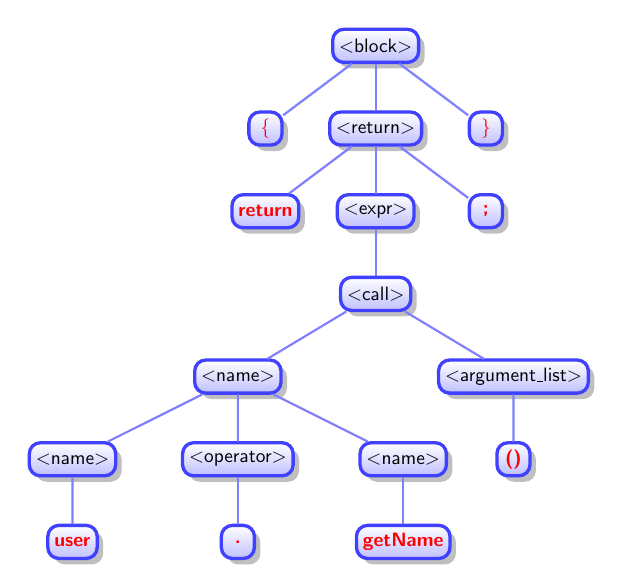
\begin{tikzpicture}[
  font=\sffamily,
  scale=0.7,
  every node/.style={top color=white, bottom color=blue!25, 
  rectangle,rounded corners, minimum size=6mm, draw=blue!75,
  very thick, drop shadow, align=center,scale=0.7},
  edge from parent/.style={draw=blue!50,thick},
  sibling distance=2cm,
  tlabel/.style={pos=0.4,right=-1pt,font=\footnotesize\color{red!70!black}},
  level 4/.style={sibling distance=5cm},
  level 5/.style={sibling distance=3cm},
]
\node{$<$block$>$}
child {node {\textcolor{red}{\textbf{$\lbrace$}}}}
child {node {$<$return$>$}
  child {node {\textcolor{red}{\textbf{return}}}}
  child {node {$<$expr$>$}
    child {node {$<$call$>$}
      child {node {$<$name$>$}
        child {node {$<$name$>$}
          child {node {\textcolor{red}{\textbf{user}}}
          }
        }
        child {node {$<$operator$>$}
          child {node {\textcolor{red}{\textbf{.}}}
          }
        } 
        child {node {$<$name$>$}
          child {node {\textcolor{red}{\textbf{getName}}}
          }
        }
      }
      child {node {$<$argument\_list$>$}
        child {node {\textcolor{red}{\textbf{()}}}
        }
      }
    }
  }
  child {node {\textcolor{red}{\textbf{;}}}
  }
}
child {node {\textcolor{red}{\textbf{$\rbrace$}}}
};
\end{tikzpicture}
%\vspace{-10pt}
\caption[Illustration of an AST in the srcML format]{Illustration of the AST of the highlighted fragment of the code presented in the \Cref{listings:srcml-xml}. The text nodes that correspond to source code are coloured red.}
\label{listings:srcml-ast}
\end{figure}


\section{\texttt{APTED} Example}
\label{sec:apted}

Another tool used in our implementation is the \texttt{APTED}\footnote{\url{http://tree-edit-distance.dbresearch.uni-salzburg.at/} one, which computes the tree edit distance between two trees. The designers of the tool define the tree edit distance as ``the minimum-cost sequence of node edit operations that transform one tree into another''}. The tool considers three edit operations, namely the \textit{insertion}, \textit{deletion} and \textit{renaming} (also called \textit{substitution} in string edit distances) of a tree node. In \Cref{listings:apted1-java,listings:apted1-xml,listings:apted1-transaction,listings:apted2-java,listings:apted2-xml,listings:apted2-transaction} we present an example of two Java source code files (\Cref{listings:apted1-java,listings:apted2-java}), that are transformed to their srcML format (\Cref{listings:apted1-xml,listings:apted2-xml}), and then to appropriate transactions in the form used by the APTED tool (\Cref{listings:apted1-transaction,listings:apted2-transaction}). As we can see, the transaction in \Cref{listings:apted2-transaction} contains 8 additional nodes, with respect to the one in \Cref{listings:apted2-transaction} (these are highlighted). Hence, the tree edit distance between these two trees, computed by the APTED tool, is 8, as there are 8 addition operations.

\begin{figure}[h]
\lstinputlisting[language=Java]{listings/APTED1.java}
\vspace{-10pt}
\caption[Summarised snippet to be compared with the snippet in \Cref{listings:apted2-java}, using the APTED tool]{Summarised snippet to be compared with the snippet in \Cref{listings:apted2-java} using the APTED tool.}
\label{listings:apted1-java}
\end{figure}

\begin{figure}[h]
\lstinputlisting[language=Java]{listings/APTED2.java}
\vspace{-10pt}
\caption[Summarised snippet to be compared with the snippet in \Cref{listings:apted1-java}, using the APTED tool]{Summarised snippet to be compared with the snippet in \Cref{listings:apted1-java}, using the APTED tool.}
\label{listings:apted2-java}
\end{figure}
\vspace{-10pt}

\begin{figure}[h]
\lstinputlisting[language=XML]{listings/APTED1.xml}
\vspace{-10pt}
\caption[srcML format of the file in \Cref{listings:apted1-java}]{AST of the file presented in \Cref{listings:apted1-java}, in the srcML format, extracted using the srcml tool.}
\label{listings:apted1-xml}
\end{figure}
\vspace{-10pt}

\begin{figure}[H]
\lstinputlisting[language=XML]{listings/APTED2.xml}
\vspace{-10pt}
\caption[srcML format of the file in \Cref{listings:apted2-java}]{AST of the file presented in \Cref{listings:apted2-java}, in the srcML format, extracted using the srcML tool.}
\label{listings:apted2-xml}
\end{figure}

\clearpage

\begin
{figure}[h]
\lstinputlisting[language=APTED,style=APTED]{listings/APTED1Transaction.txt}
\vspace{-10pt}
\caption[APTED transaction for the file in \Cref{listings:apted1-xml}]{Transaction in the form used by the APTED tool, for the file presented in \Cref{listings:apted1-xml}.}
\label{listings:apted1-transaction}
\end{figure}
\vspace{-20pt}

\begin{figure}[h]
\lstinputlisting[language=APTED,style=APTED]{listings/APTED2Transaction.txt}
\vspace{-10pt}
\caption[APTED transaction for the file in \Cref{listings:apted2-xml}]{Transaction in the form used by the APTED tool, for the file presented in \Cref{listings:apted2-xml}.}
\label{listings:apted2-transaction}
\end{figure}
\vspace{-30pt}

\section{\texttt{Artistic Style} Example}
\label{sec:artistic-style}

In order to increase the readability of our system's generated snippets, we make use of the \textit{Artistic Style} formatter. This is a commonly used formatter, that supports several languages, including the Java language. We set its \texttt{style} option to the \texttt{java} one, which is used for Java source code files. The way this tool works is straightforward, and thus we only provide an example in \Cref{listings:astyle-before,listings:astyle-after}, without any further analysis.

\begin{figure}[!h]
\lstinputlisting[language=Java]{listings/AstyleBefore.java}
\vspace{-10pt}
\caption[Snippet before the application of the Artistic Style formatter]{Snippet before the application of the Artistic Style formatter.}
\label{listings:astyle-before}
\end{figure}
\vspace{-20pt}

\begin{figure}[H]
\lstinputlisting[language=Java]{listings/AstyleAfter.java}
\vspace{-10pt}
\caption[Snippet after the application of the Artistic Style formatter]{The snippet presented in \Cref{listings:astyle-before}, after the application of the Artistic Style formatter to it.}
\label{listings:astyle-after}
\end{figure}
\vspace{-30pt}

\chapter{Summarisation Specifics}
\label{chap:summarisation-specifics}

\section{Summarisation Pseudocodes}
\label{sec:summarisation-pseudocodes}

One of the basic steps of the summarisation algorithm is the one where the statements are classified to API and to non-API ones. In order to decide on whether a statement belongs to the first ones or to the latter ones, the algorithm needs to be fed with the name of the API methods, that are called in the snippet to be summarised. As we see in \Cref{algorithms:statements-classifier}, the \texttt{ClassifyStmts} function then takes the tree of the source code to be summarised, as well as these names, as its input parameters, in order to classify the statements. The process followed is analysed below:

\begin{itemize}
\item In \textit{Lines 2} and \textit{3} the function initialises the two lists that are going to store the API and the non-API statements, respectively.
\item In \textit{Line 4} the function iterates over the tree in document order (also called \textit{pre-order traversal}\footnote{\url{https://en.wikipedia.org/wiki/Tree_traversal}}).
\item \textit{Line 5} checks whether a node\footnote{In this section, we use the term ``node'' to indicate element nodes in the xml file.} is the root of a \textit{statement}, as these are defined by the srcML format (e.g. \texttt{decl\_stmt}, \texttt{return}, etc.).
\item In \textit{Lines 6} and \textit{7} the function checks whether the nodes that satisfy the condition in \textit{Line 5} contain an API call in their subtree. Based on the latter decision, they are appended to the appropriate list.
\item In \textit{Line 11} it checks whether a node is the root of a \textit{condition}, as these are once more defined by the srcML format (e.g. \texttt{condition}, \texttt{control}, etc.).
\item \textit{Line 12} checks whether the parent node of a node that satisfies the condition in \textit{Line 11}, contains an API call. If so, the node is added to the list where the API statements are stored. Justifying this part of the algorithm, we firstly point out that each node that is a root of a condition statement (e.g. \texttt{condition}, \texttt{control}, etc.), has a parent that is a control\footnote{To avoid confusion, here we are talking about decision-making and looping statements (see \url{https://docs.oracle.com/javase/tutorial/java/nutsandbolts/flow.html}), rather than about the \texttt{control} element, used in the srcML format.} statement (e.g. \texttt{if}, \texttt{for}, etc.), in the srcML format. In addition to that, if -the subtree of- a control statement contains an API call, then we should also keep -the subtree of- its condition(s)\footnote{A hidden point here is that the srcML format handles the \texttt{case} statements of a \texttt{switch} statement in a similar manner to \texttt{conditions}, and hence we consider them as conditions, too.} in the summarised code. Based on this, we may classify the condition statements using their associated control statements classification information. Moreover, our decision to exclude the \texttt{else} statement of the condition in \textit{Line 12} stems from the fact that there is no need to add a condition statement into the corresponding list, in case it is a non-API statement, as the first is going to be removed, too, in case its associated control block is removed.
\item Finally, \textit{Lines 15-17} check whether -the subtree of- a control statement contains an API call, and if not, this is added to the appropriate list. Note that there is no need to add a control statement into the corresponding list, in case it contains an API call, as all the API statements of its subtree are going to be added to the list, as either \textit{statement} or \textit{condition} nodes.
\end{itemize}

\begin{algorithm}
\small
\caption[Statements Classifier]{Statements Classifier}
\label{algorithms:statements-classifier}
\begin{algorithmic}[1]
\Procedure{ClassifyStmts}{$tree$, $API\_calls$}
	\State $API\_stmts \leftarrow 0$
	\State $non\_API\_stmts \leftarrow 0$
	
	\ForAll{$node \in tree$}
	\Comment{Iterate over the $tree$ in document order}
		\If{$node$ is a $statement$}
			\If{$node.subtree$ contains an $API\_call \in API\_calls$}
				\State $API\_stmts \leftarrow API\_stmts \cup node$
			\Else
				\State $non\_API\_stmts \leftarrow non\_API\_stmts \cup node$
			\EndIf
		\ElsIf{$node$ is a $condition$}
			\If{$node.parent.subtree$ contains an $API\_call \in API\_calls$}
				\State $API\_stmts \leftarrow API\_stmts \cup node$
			\EndIf
		\ElsIf {$node$ is a $control$}
			\If{$node.subtree$ does not contain any $API\_call \in API\_calls$}
				\State $non\_API\_stmts \leftarrow non\_API\_stmts \cup node$
			\EndIf
		\EndIf
	\EndFor
	\Return $API\_stmts$, $non\_API\_stmts$
\EndProcedure
\end{algorithmic}
\end{algorithm}

\clearpage

\section{Summarised Snippets}
\label{sec:summarised-snippets}

In this section we are going to show the effect of the summarisation algorithm to the Java snippets it is applied to. Indicative examples are shown for features including the variables type resolution, the literals replacement, as well as the addition of descriptive comments, which are added either in case of empty blocks, or in snippets where variables that are declared in API statements are used in non-API statements (which are removed from the summarised snippet). We also provide an example which mainly shows the removal of any non-API statements.
\vspace{10pt}

\noindent
\textsc{A. Variables Type Resolution}
\vspace{5pt}

The summarisation algorithm is able to resolve the type of -almost\footnote{A limitation of our approach when resolving variables type is that we do not take into account the scope of a variable. Although this may lead to an incorrect type resolution, this occurs in rare cases only.}- any variable used in the snippet, in case this information is available in the original source code file. An example of this feature is shown in \Cref{listings:resolve-types-org,listings:resolve-types-sum}.

\begin{figure}[h]
\lstinputlisting[language=Java]{listings/ResolveTypesOrg.java}
\vspace{-10pt}
\caption[Java snippet with unresolved variables]{Java snippet with unresolved variables.}
\label{listings:resolve-types-org}
\end{figure}
\vspace{-20pt}

\begin{figure}[H]
\lstinputlisting[language=Java]{listings/ResolveTypesSum.java}
\vspace{-10pt}
\caption[Summarised snippet, after type resolution]{Summarised snippet of the source code presented in \Cref{listings:resolve-types-org}, after the type resolution.}
\label{listings:resolve-types-sum}
\end{figure}
\vspace{-20pt}

\clearpage

\noindent
\textsc{B. Literals Replacement}
\vspace{5pt}

One of the features of the summarisation algorithm is that it replaces the literals, as these are defined in the srcML format, with their types. This includes numbers, strings or even booleans. For instance, the snippet presented in \Cref{listings:literals-org} is summarised to the one shown in \Cref{listings:literals-sum}.

\begin{figure}[h]
\lstinputlisting[language=Java]{listings/LiteralsOrg.java}
\vspace{-10pt}
\caption[Java snippet, before literals' replacement]{Java snippet, before the literals replacement.}
\label{listings:literals-org}
\end{figure}

\vspace{-20pt}

\begin{figure}[h]
\lstinputlisting[language=Java]{listings/LiteralsSum.java}
\vspace{-10pt}
\caption[Summarised snippet, after literals' replacement]{Summarised snippet of the source code in \Cref{listings:literals-org}, after the replacement of literals with their srcML type.}
\label{listings:literals-sum}
\end{figure}

\noindent
\textsc{C. Addition of Descriptive Comments inside Empty Blocks}
\vspace{5pt}

A feature of the summarisation algorithm that aims to improve the readability of the mined snippets, is the addition of descriptive comments, in case of empty blocks. The idea behind that is analysed in \cite{Borges:2014}, while an example that shows the effect of this feature is presented in \Cref{listings:empty-block-org,listings:empty-block-sum}.

\begin{figure}[h]
\lstinputlisting[language=Java]{listings/EmptyBlockOrg.java}
\vspace{-10pt}
\caption[Java snippet, with an empty block]{Java snippet with an empty block, before adding a descriptive comment.}
\label{listings:empty-block-org}
\end{figure}

\vspace{-20pt}

\begin{figure}[!h]
\lstinputlisting[language=Java]{listings/EmptyBlockSum.java}
\vspace{-10pt}
\caption[Summarised snippet, with a descriptive comment inside the empty\protect\\block]{Summarised snippet of the source code presented in \Cref{listings:empty-block-org}, after the addition of a descriptive comment inside the empty block.}
\label{listings:empty-block-sum}
\end{figure}

\clearpage

\noindent
\textsc{D. Addition of Descriptive Comments for Variables Declared in API Statements that are Used Only in non-API Statements}
\vspace{5pt}

This is a feature that adds a novelty to our summarisation algorithm. It is based on a similar feature introduced by \nolink{\citeauthor{Buse:2012}} in \cite{Buse:2012}. However, in our case, we make use of the API statements, as well as of the non-API statements of the source code to be summarised. That is, we check whether an API statement declares a variable that is then used only in non-API statements (which are removed in the summarised version). If so, we add a descriptive comment for the declared variable. The effect of this feature is shown in \Cref{listings:forward-comment-org,listings:forward-comment-sum}.

\begin{figure}[h]
\lstinputlisting[language=Java,style=Java]{listings/CommentsOrg.java}
\vspace{-10pt}
\caption[Java snippet without descriptive comments]{Java snippet without descriptive comments. The API method calls are highlighted.}
\label{listings:forward-comment-org}
\end{figure}

\vspace{-20pt}

\begin{figure}[h]
\lstinputlisting[language=Java,style=Java]{listings/CommentsSum.java}
\vspace{-10pt}
\caption[Summarised snippet with descriptive comments]{Summarised snippet of the source code presented in \Cref{listings:forward-comment-org}, after the addition of descriptive comments. The API method calls are highlighted.}
\label{listings:forward-comment-sum}
\end{figure}


An indicative example that reveals the efficiency of the summarisation algorithm in case of large snippets is presented in \Cref{listings:without-summariser,listings:with-summariser}.

\begin{figure}[h]
\lstinputlisting[language=Java,style=Java]{snippets/WithoutSummariser.java}
\vspace{-10pt}
\caption[Client code without the summariser]{Client code without the summariser. The API calls are highlighted.}
\label{listings:without-summariser}
\end{figure}

\begin{figure}[h]
\lstinputlisting[language=Java,style=Java]{snippets/WithSummariser.java}
\vspace{-10pt}
\caption[Client code with the summariser]{Summarised version of the client code presented in \Cref{listings:without-summariser}. The API calls are highlighted.}
\label{listings:with-summariser}
\end{figure}
\chapter{Evaluation Specifics}
\label{chap:evaluation-specifics}

\section{Computing the Snippet-Based Metrics}
\label{sec:snippet-based-metrics}

The process followed in order to compute the snippet-based metrics, is analysed below:

\begin{enumerate}
\item For each source code file (mined snippets and examples), we extract a sequence of tokens, using a Java code tokeniser, that has been implemented as a previous work of our team. The Java Tokenizer makes use of the Eclipse JDT, in order to extract a list of tokens from a serialised version of a Java source code. We have proceeded to a few modifications on the existing version of the Tokenizer, in order to be able to tokenise multiple files, and to write the output to a \texttt{.json} file. An example that shows the tokens extracted from a Java source code is presented in \Cref{listings:java-tokenizer-code,listings:java-tokenizer-tokens-org}.
\item Having extracted a \texttt{.json} file where the tokens of the mined snippets/examples are stored, we proceed to some basic preprocessing; this includes the removal of any symbols (e.g. brackets, semicolons, etc.), as well as of any comments and Javadocs. Moreover, we replace any literals (e.g. Strings, numbers, etc.) with their srcML type, in order to be able to fairly evaluate the summarisation algorithm, which includes this step. The revised list of tokens for the example presented in \Cref{listings:java-tokenizer-code} is shown in \Cref{listings:java-tokenizer-tokens-rev}.
\item For each snippet, we check whether an example contains the same API calls (it may contain additional ones, but this is not a problem). If so, we use the snippet-based metrics defined in \Cref{sec:evaluation-metrics}. In case multiple examples match to the snippet, with respect to its API calls, we match the snippet to the one that maximises the number of their common tokens.
\end{enumerate}

\begin{figure}[ht]
\lstinputlisting[language=Java]{listings/JavaTokenizerCode.java}
\vspace{-10pt}
\caption[Java snippet to be tokenised by the Java Tokenizer]{Java snippet to be tokenised by the Java Tokenizer.}
\label{listings:java-tokenizer-code}
\end{figure}

\vspace{-10pt}

\begin{figure}[ht]
\lstinputlisting{listings/JavaTokenizerTokensOrg.txt}
\vspace{-10pt}
\caption[Java tokens extracted using the Java Tokenizer]{Java tokens extracted from the Java source code presented in \Cref{listings:java-tokenizer-tokens-org}, using the Java Tokenizer.}
\label{listings:java-tokenizer-tokens-org}
\end{figure}

\vspace{-10pt}

\begin{figure}[H]
\lstinputlisting{listings/JavaTokenizerTokensRev.txt}
\vspace{-10pt}
\caption[Revised list of Java tokens]{Revised list of Java tokens for the Java source code presented in \Cref{listings:java-tokenizer-tokens-org}, after the preprocessing step.}
\label{listings:java-tokenizer-tokens-rev}
\end{figure}


\section{Experiment 1}
\label{sec:exp1-qualitative}

\begin{figure}[!h]
\lstinputlisting[language=Java]{snippets/Exp1Ex1Org.java}
\vspace{-10pt}
\caption[Snippet ranked first by the $RemUniqNaivNoSum$ version of the system]{Snippet ranked first by the $RemUniqNaivNoSum$ version of the system.}
\label{listings:exp1-ex1-org-java}
\end{figure}

\vspace{-10pt}

\begin{figure}[!h]
\lstinputlisting[language=Java]{snippets/Exp1Ex1Sum.java}
\vspace{-10pt}
\caption[Snippet ranked first by the $RemUniqNaivSum$ version of the system]{Snippet ranked first by the $RemUniqNaivSum$ version of the system. This snippet is a summary of the one presented in \Cref{listings:exp1-ex1-org-java}.}
\label{listings:exp1-ex1-sum-java}
\end{figure}


\begin{figure}[!h]
\lstinputlisting[language=Java]{snippets/Exp1Ex2Org.java}
\vspace{-10pt}
\caption[Random snippet mined by the $RemUniqNaivNoSum$ version of the system]{Random snippet mined by the $RemUniqNaivNoSum$ version of the system.}
\label{listings:exp1-ex2-org-java}
\end{figure}

\vspace{-10pt}

\begin{figure}[!h]
\lstinputlisting[language=Java]{snippets/Exp1Ex2Sum.java}
\vspace{-10pt}
\caption[Random snippet mined by the $RemUniqNaivSum$ version of the\protect\\system]{Random snippet mined by the $RemUniqNaivSum$ version of the system. This snippet is a summary of the one presented in \Cref{listings:exp1-ex2-org-java}.}
\label{listings:exp1-ex2-sum-java}
\end{figure}

\clearpage

\section{Experiment 2}
\label{sec:exp2-qualitative}

\begin{figure}[!h]
\lstinputlisting[language=Java]{snippets/Exp2RemUniqueTopExamples.java}
\vspace{-10pt}
\caption[Top 5 snippets mined by the $RemUniqNaivSum$ version of the system]{The top 5 snippets, with respect to their support, mined by the $RemUniqNaivSum$ version of the system.}
\label{listings:exp2-rem-unique-top-examples}
\end{figure}

\vspace{-10pt}

\begin{figure}[!h]
\lstinputlisting[language=Java]{snippets/Exp2KeepUniqueTopExamples.java}
\vspace{-10pt}
\caption[Top 5 snippets mined by the $KeepUniqNaivSum$ version of the system]{The top 5 snippets, with respect to their support, mined by the $KeepUniqNaivSum$ version of the system.}
\label{listings:exp2-keep-unique-top-examples}
\end{figure}

\clearpage

\section{Experiment 3}
\label{sec:exp3-qualitative}

\begin{figure}[!h]
\ffigbox
{%
  \begin{subfloatrow}[2]
  \ffigbox[\FBwidth]
    {\caption{}\label{listings:k-medoids-top-sequences}}{\lstinputlisting{listings/KMedoidsTopSequences.txt}}
  \hspace{1em}%
  \ffigbox[\FBwidth]
    {\caption{}\label{listings:HDBSCAN-top-sequences}}{\lstinputlisting{listings/HDBSCANTopSequences.txt}}
  \end{subfloatrow}}
  {\caption[Top 10 sequences mined by the $KeepUniqKMedoidsSum$, and the\protect\\$KeepUniqHDBSCANSum$ versions of the system]{The top 10 sequences, with respect to their support, mined (\subref{listings:k-medoids-top-sequences}) by the $KeepUniqKMedoidsSum$, and (\subref{listings:HDBSCAN-top-sequences}) by the $KeepUniqHDBSCANSum$ version of the system, that leverage the $k$-medoids and the HDBSCAN clustering techniques, respectively.}
\label{fig:clustering-top-sequences}}
\end{figure}

\begin{figure}[!h]
\lstinputlisting[language=Java]{snippets/Top5SnippetsHDBSCAN.java}
\vspace{-10pt}
\caption[Top 5 snippets mined by the $KeepUniqHDBSCANSum$ version of the system]{The top 5 snippets, with respect to their support, mined by the $KeepUniqHDBSCANSum$ version of the system.}
\label{listings:exp3-hdbscan-top-snippets}
\end{figure}

\begin{figure}[!h]
\lstinputlisting[language=Java]{snippets/Top5SnippetsKMedoids.java}
\vspace{-10pt}
\caption[Top 5 snippets mined by the $KeepUniqKMedoidsSum$ version of the system]{The top 5 snippets, with respect to their support, mined by the $KeepUniqKMedoidsSum$ version of the system.}
\label{listings:exp3-kmedoids-top-snippets}
\end{figure}

\clearpage

\section{Experiment 5}
\label{sec:exp5-qualitative}

\begin{figure}[!h]
\lstinputlisting[language=Java,style=Java]{snippets/WellMatchedHDBSCAN.java}
\vspace{-10pt}
\caption[Additional tokens revealed when mining snippets instead of sequences]{A snippet mined by the $KeepUniqHDBSCANSum$ version of the system, that has been matched to a handwritten example. The common tokens between the snippet and the handwritten examples it matches to are highlighted; the sequence-tokens are only coloured, while the additional snippet-tokens are moreover encircled, and show the additional information revealed to the developers when presenting snippets instead of sequences.}
\label{listings:exp5-well-matched-hdbscan}
\end{figure}

\begin{figure}[!h]
\lstinputlisting[language=Java,style=Java]{snippets/NotMatchedHDBSCAN.java}
\vspace{-10pt}
\caption[Mined snippet not matched to any handwritten example]{A snippet mined and placed in the second position by the $KeepUniqHDBSCANSum$ version of the system. It has not been matched to any handwritten example, although it is supported by $70$ source code files in the mined dataset. In fact, there is no handwritten example that covers the \texttt{setOauthConsumer} method of the \texttt{Twitter4J} API, which is considered as one of the most popular methods of the API. This shows that our system may be well used in order to augment the documentation of an API with new examples.}
\label{listings:exp5-not-matched-hdbscan}
\end{figure}


% Bibliography style
\bibliographystyle{unsrtnat}

%% If you want the bibliography single-spaced (which is allowed), uncomment
%% the next line.
% \singlespace

%% Specifies the bibliography file
\bibliography{references}

\end{document}
